% !TEX root = ../thesis_main.tex
%
%
%
%%%% --- * --- %%%%	
\chapter{Background}
\label{intro_chapter}
\label{nuclear_chapter}
\note[jbnn]{For sure you should ask for the electronic grammar corrections :) !!
\\
I hope you've already done so.
}
\note[jbnn]{I will write more on 5 and 6 soon and provide Hayen2021~\cite{Hayen2021}. It is quite reasonable to take the approach
of saying `the important parts for the experiment can be described schematically' and 'the details were part of another thesis'
and I can help with those important parts.}
\note[jbnn]{hi Melissa,
\\...\\
explaining $f_A/f_V$ gives a chance to cite Leendert's recent work~\cite{Hayen2021} on a radiative correction in G-T decay, and
\\...\\
an assortment of other small corrections to mirror decays
(his collaboration with Cirigliano is working on an additional correction in the neutron...).
\\
His Table I and Fig. 5 have results for 37K. Since $f_A/f_V$ is closer to 1 in our case, I think because the weak magnetism is small (and we-- i.e. Dan and Ben et al-- had already done a correct incorporation of $f_A/f_V$ and such, not overcounting a term LH mentions was done in the literature) , in the end it has turned out we agree with his interpretation of our 37K result. 
\\...\\
A difference not enough for you to worry about. But this is the best place to find $f_A/f_V$.
}
%
Within nature, there exist four fundamental forces governing the interactions of particles with one another:  electromagnetism, the nuclear weak force, the nuclear strong force, and gravity.  This work seeks to probe the nature of the weak nuclear force on its most fundamental level through observations of beta decay, a process which results directly from the action of the weak nuclear force.  Through kinematic observations of the decay products, much can be learned about the form of the weak nuclear force's coupling, through which beta decay proceeds.  Prior experiments have shown that this coupling is dominated by a combination of operators that behave as vectors and axial-vectors under Lorentz transformation, however 
%vector and axial-vector operators, but 
the possibility of a non-dominant contribution from other types of operators, such as scalars and tensors, cannot be ruled out entirely.  This is the domain of precision measurements.  

\section{Introduction}
\label{section:intro}
Within our present understanding of physics, there are four fundamental forces governing the interactions of particles with one another:  electromagnetism, the nuclear weak force, the nuclear strong force, and gravity.  These forces are considered to be distinct from one another by virtue of their differing behaviours, however attempting to unify them within a single theoretical framework has been a major focus of later 20th- and early 21st century physics to date.  The effort has been met with only partial success, and the resulting theoretical framework is collectively known as the \ac{SM}.

The standard model provides a quantum mechanical description for
the behaviour of three of the four fundamental forces:  electromagnetism, the nuclear weak force, and the nuclear strong force.  The \ac{SM} notably does not describe gravitational processes --- despite extensive efforts, the gravitational force has thus far defied all attempts to describe it in a fully quantum mechanical way, though this remains an active field of research.  

%
Each force has its own specific mediating particle(s) which couple only to a particular type of (generalized) charge, and therefore interact only with particles that possess that charge.  For example, the gravitational charge is \emph{mass}, and (at least within a simplified particle physics model) gravity acts only on objects that possess mass.~\aside{Can I turn this into a footnote?  It's not true because the curvature of spacetime also affects photon trajectories, and there even exist (unstable) (quasi-?) bound states comprised *only* of photons, as in e.g. Aichelburg-Sexl.}  With only a single type of charge and no negative masses, the gravitational force can only ever be attractive.
%
By constrast, the electromagnetic force couples to both positive and negative electric charges, and can produce both attractive and repulsive forces.  Both the electromagnetic and gravitational forces are mediated by massless force-carrying particles (the photon and still-theoretical graviton, respectively), a property which implies that the amount of flux per unit solid angle is constant over all distance scales, and Gauss's Law holds true.

\begin{figure}[h!t!b!]
	\centering
	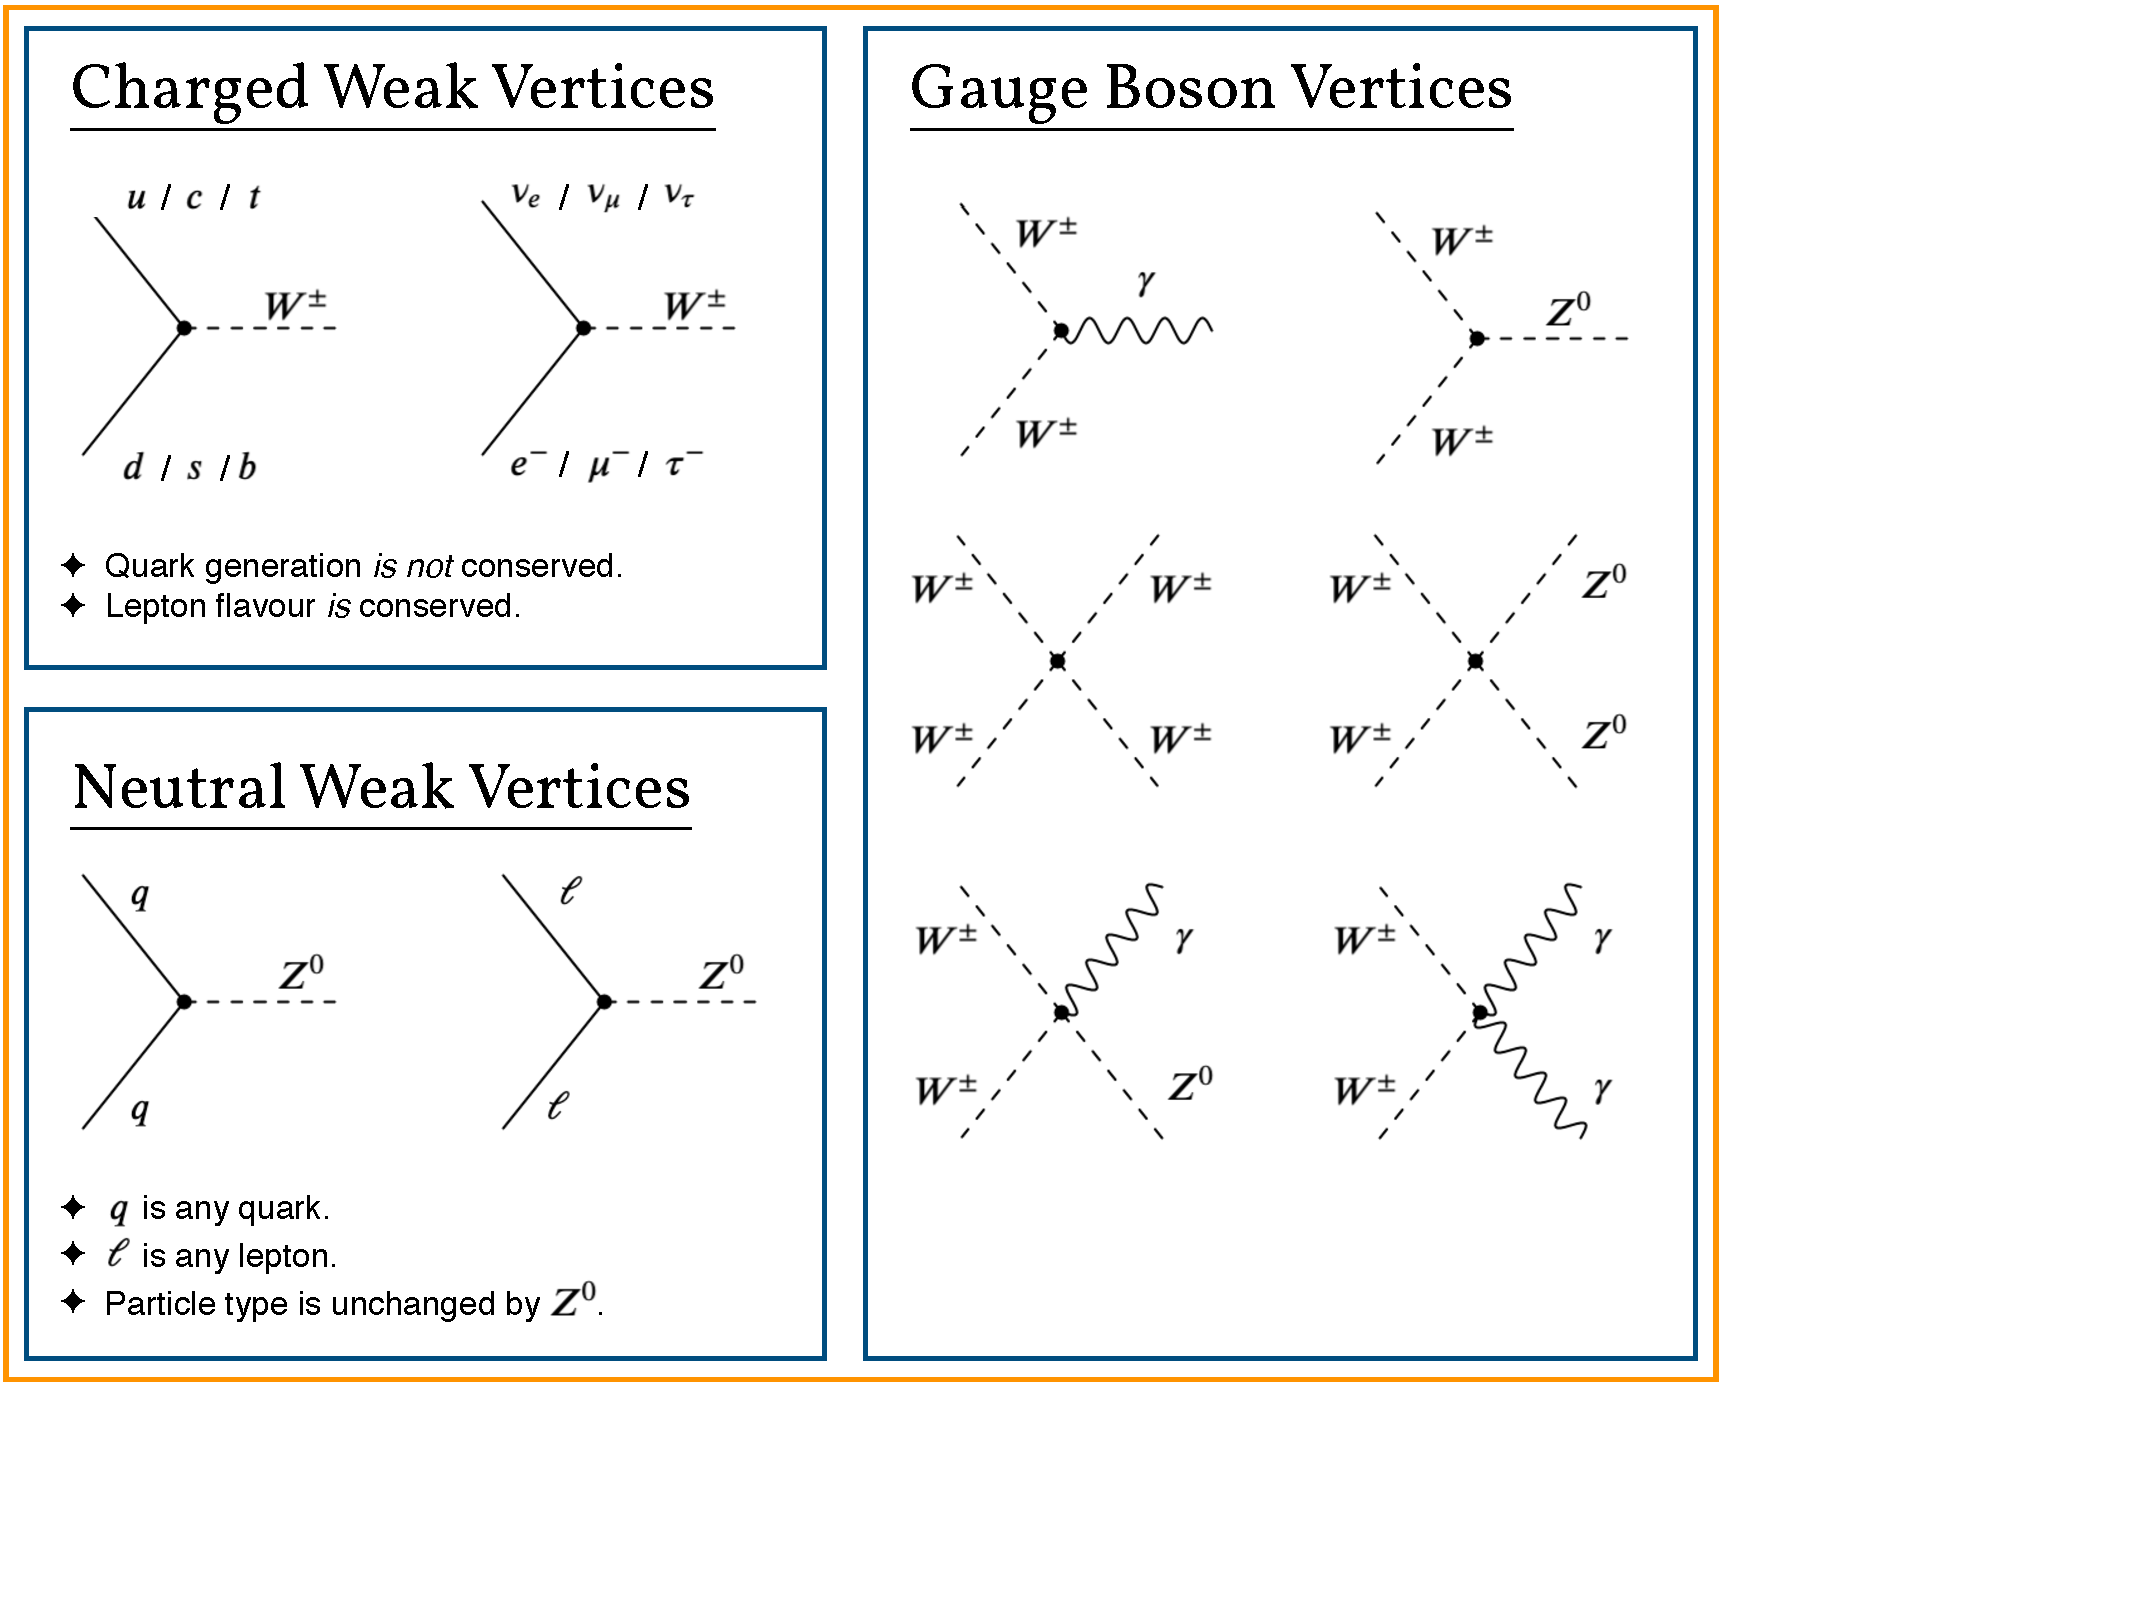
\includegraphics[width=1.0\linewidth]{Figures/VertexFeynmanDiagrams.pdf}
%	\note[tag]{Fix Feynman diagram vertex placeholder figure.}
	\caption[An exhaustive list of weak vertices]{An exhaustive list of weak vertices.  All possible Feynman diagram vertices involving $W^+$, $W^-$, or $Z^0$ bosons are shown, and the usual rules apply.  These vertices show the types of interactions that can occur between the bosons mediating the weak force, and other types of particles.  Only the fundamental vertices are shown, meaning that these diagrams are in some sense incomplete.  At the energy scales available in everyday life, the $W$ and $Z$ bosons act only as an intermediary between two such vertices.}	
	\label{fig:feynmandiagrams_general}
\end{figure}

In the case of the nuclear weak force, which will be the primary concern within this thesis, 
the notion of generalized charge is no longer entirely straightforward to apply.
We must rely instead on a list of allowed Feynman diagram vertices to describe the types of interaction that are possible (see Fig.~\ref{fig:feynmandiagrams_general}).  We note that the weak force involves three mediating particles --- $W^+$, $W^-$, and $Z^0$ bosons --- and these mediators can interact with both (anti-)quarks and (anti-)leptons.  The $W^+$ and $W^-$ particles also carry electric charge, which must be separately conserved in any interaction,~\aside{(wait, is that true?  what about with the photon vertex? ....I think it's fine.....} but the $Z^0$ is electrically neutral.  All three are massive, which implies that the strength of the weak force falls off more rapidly as distance increases, and Gauss's Law does not apply. 


With a comparatively large number of possible vertex types, it can be challenging to develop an intuition about the behaviour of the weak force. 
Perhaps the most well known physical behaviour that arises from the nuclear weak force is beta decay. 
Indeed, beta decay
offers one of the most readily accessible experimental windows to the workings of the nuclear weak force.

Although it is now generally well understood, beta decay still presents a unique opportunity for precision measurements to search for exotic physics beyond the Standard Model within the weak coupling.
By observing the kinematics and angular correlations involved in the decay process, one gains access to a wealth of information about the 
laws underpinning the decay process, and the weak force as a whole.  



%%%% --- * --- %%%%	
\section{A Historical Look at Beta Decay and the Weak Interaction}

We consider the historical development of our scientific understanding of beta decay and the nuclear weak force.  This is a historically rich topic, and a full discussion is beyond the scope of this document, however we shall attempt to touch on some highlights.

Radioactivity was first observed in 1896 by Henri Becquerel in uranium, and this landmark discovery set off a flurry of activity in the field~\cite{becquerel1896}.
Ernest Rutherford noted in 1899 that the particles emitted by a sample of uranium could be classified into two groups based on how readily they were absorbed in materials -- alpha particles are easily absorbed, while beta particles are more penetrating~\cite{rutherford1899}.  A third and even more penetrating type of radioactive emission was observed in 1900 by Paul Villard, who made no attempt to give it a name -- but within a few years, Rutherford's naming convention had been applied and this third type of particle became known as a gamma ray~\cite{villard1900}\cite{rutherford1903}.  

\note{Rutherford discovered that:  half-life.  [76]=E. Rutherford, \emph{Phil. Mag.} \textbf{49}, 1, 1900.  Thorium.  Rn220.  ...but also, *I* got this from Abraham Pais.}

When, in 1900, Becquerel measured the charge-to-mass ratio of emitted beta ($\beta^-$) radiation and found that it was the same as that of the electron, he proposed that these must be the same particle~\cite{becquerel1900},~\aside{I think.  Also, I think that's the right citation..} and in 1903~\aside{or possibly 1901?} Rutherford and Soddy demonstrated that the processes of alpha and beta decay both transmute the original chemical element into another\cite{rutherfordsoddy1903}.


Despite these early successes, in 1911 Lise Meitner and Otto Hahn noticed that beta particles are emitted with a variety of different kinetic energies,~\aside[tag]{citation needed} and in 1914 James Chadwick
%%~\aside{citation needed.  also, maybe it was a bunch of people, 1914-1927.  
%%\\
%%Chadwick's original:  Chadwick, J. (1914). "Intensitätsverteilung im magnetischen Spektren der β-Strahlen von Radium B + C". Verhandlungen der Deutschen Physikalischen Gesellschaft (in German). 16: 383–391.  
%%\\
%%Maybe also Charles Drummond Ellis?  
%%\\
%%Ellis and Wooster:  Ellis, C. D.; Wooster, W. A. (1927). "The Continuous Spectrum of β-Rays". Nature. 119 (2998): 563–564. doi:10.1038/119563c0. S2CID 4097830.  } 
demonstrated that energies of emitted beta particles formed a continuous distribution.  The physics community was baffled for years by the fact that it seemed impossible to predict the energy of a beta particle emitted by a particular process;  if the emitted beta simply took on the difference in energy between the initial and final states, then surely that energy should be a fixed, unchanging value for a paricular transition. 

%should be a fixed amount of energy for a given transition.  
Finally, in 1930, a frustrated Wolfgang Pauli famously proposed that if an additional small, neutral, difficult to detect particle were emitted simultaneously with the beta and allowed to carry away a varying amount of energy, then this accounting trick could account for the continuous beta energy spectrum.
%could account for the continuous beta energy spectrum, by carrying away whatever fraction of the
%This new particle was dubbed a ``neutron'' 
He named this particle a ``neutron'' -- though today we refer to that same particle as a(n) ``(anti-)neutrino,'' and use the name ``neutron'' for an entirely different particle\cite{PauliNeutrino1978}.  \aside{Fermi renamed it, because Italian.}

%When Enrico Fermi offered a quantitative description of 
Pauli's 1930 insight paved the way for Enrico Fermi to propose a quantitative description of the nuclear weak force and the beta decay processes resulting from it.  He modeled the weak force as a contact interaction with zero range --- a very good approximation.  After being rejected by \emph{Nature} in 1933, Fermi's seminal theory of beta decay was published in both Italian and German journals the following year \cite{AbrahamPais} \cite{Fermi1934Italian} \cite{Fermi1934German}.
%\aside[done]{Citation is:  Pais, Abraham (1986). Inward Bound. Oxford: Oxford University Press. p. 418. ISBN 0-19-851997-4. \cite{AbrahamPais} }  
Because of its powerful predictive ability together with its generalized quantum mechanical approach, Fermi's model forms the basis upon which modern beta decay calculations have been built.  With one of its major results, now commonly known as Fermi's Golden Rule, still routinely used, the introduction of Fermi's model arguably marks the beginning of our modern understanding of beta decay.

The mid 1930s was a busy time 
%1934 was a busy year 
for our understanding of beta decay.  In addition to the publication of Fermi's model in 1934, this year also marks the first discovery of $\beta^+$ radiation, for which Irène and Frédéric Joliot-Curie later received a Nobel prize, and the proposal by Gian-Carlo Wick of the electron capture mechanism for beta decay.  
The electron capture theory was fleshed out further in 1935-1936 by Yukawa and Sakata\aside{and others?},\aside{Yukawa and Sakata first names?} and first observed in 1937 by Luis Alvarez.  Meanwhile, in 1936 George Gamow and Edward Teller improved upon Fermi's model by including a mechanism to potentially change the nuclear spin\cite{GamowTeller}, and to this day, beta decay transitions are still routinely classified as following Fermi or Gamow-Teller (or mixed) selection rules.

%~\aside{omg, I can't just give first names for only the non-Asian people...}
%\note[tag]{Gamow-Teller in 1936\cite{GamowTeller}. }
%1934 was also the year when Wick proposed the electron capture mechanism for beta decay, later observed by Luis Alvarez in 1937.  \aside{Yukawa and others totes helped flesh out the theory behind E.C.  Or possibly they proposed it first?  who even knows.}
Over the next few years, developments within the field of nuclear physics were largely directed elsewhere, but beta decay returned to scientific prominence with T. D. Lee and C. N. Yang's 1956 suggestion~\aside[tag]{Probably point out that this thing is the basis for the model of the weird-ass currents I'm looking for.  They made a (nucleon-level) Hamiltonian with *everything*.} 
that, contrary to the community's prior expectation, parity may not be conserved within beta decay processes\cite{LeeYang}.
~\aside{their hamiltonian operates at the nucleon level, because they hadn't discovered quarks yet.  also, this is the basis for where we're going with this experiment.  shows all possible Lorentz-invariant contributions to the thingy. V,A,S,T,P.  I don't think they knew about W and Z bosons either.}  The proposition was rapidly put to the test by C.S. Wu's landmark 1957 measurement of $^{60}$Co, confirming that beta decay violates parity conservation and simultaneously paving the way for the Nobel prize to be awarded to Lee and Yang that same year~\cite{wu}.~\aside{nobel prize citation?}
~\aside{For a while everyone thought it was S,T.  But it turns out it's V,A.  Ben cites these guys for S,T:  \cite{RustadRuby1955tensor}\cite{BurgyEpstein1957scalartensor}.  though, the one article is before Wu. Also, I can't access these things.  Look at JTW's refs maybe..}
%\note{... a discovery which earned Lee and Yang a Nobel prize.  Wu's discovery earned Lee and Yang the 1957 Nobel Prize.}

Subsequent experiments demonstrated that not only was parity non-conserved in a beta decay transition, it is (as near as we can collectively tell) \emph{maximally} violated.  \aside{cite someone for maximal parity violation.}
Though early experiments suggested that the couplings were likely comprised of 
%so-called 
scalar and tensor interactions,\aside{cite someone for S,T !  John suggests 6He $\abetanu$ for the tensor.} Feynman and Gell-Mann first postulated the correct $(V-A)$ form of the interaction in 1958 by invoking an analogy with the photon, and this was eventually borne out by experimental evidence\cite{FeynmanGellMann1958}.  (See Sec.~\ref{sec:SMandBeyond} for further discussion on the form of weak interaction couplings.)
\aside{cite someone for $(V-A)$ evidence}

In the following years, the theory behind the nuclear weak force was developed further, and eventually merged with the theory of electromagnetism as the electroweak force.  The framework for \ac{QED} had already been largely developed between 1946 and 1950 by Shinichiro Tomonaga, Julian Schwinger, Richard Feynman, and others.  The theory was fully covariant, meaning that it behaves properly under a Lorentz transformation.  The work of Schwinger, and independently, Tomonaga, developed much of the methodology behind renormalization, which is now considered to be a mathematical necessity in any modern quantum field theory\cite{tomonaga1946}\cite{schwinger1948covariant}\cite{feynman1949spacetime}\cite{feynman1949positrons}\cite{feynman1950}\cite{dyson1949theories}.  ~\aside{QED as a "template" for other theories.}


\note{From Wikipedia:  ``In 1957, Robert Marshak and George Sudarshan and, somewhat later, Richard Feynman and Murray Gell-Mann proposed a $V-A$ Lagrangian for weak interactions.''
\\...\\
``In the Standard Model, the $W^\pm$ and $Z^0$ bosons, and the photon, are produced through the spontaneous symmetry breaking of the electroweak symmetry SU(2) × U(1)Y to U(1)em, ...''
}

Following the success of QED, there was a push from the physics community to create a similar theory to model the nuclear weak force.  
%
Lee and Yang, and Feynman and Gell-Mann, produced two notable early examples of a weak force Lagrangian written, like the theory of electromagnetism, in terms of Lorentz-transforming currents\cite{LeeYang}\cite{FeynmanGellMann1958}.  Yang and Mills took a more mathematical approach, and their 1954 non-abelian gauge theory \cite{YangMills1954} lies at the foundation of electroweak unification.  
%

In 1961, Sheldon Glashow extended some of Schwinger's work to model the nuclear weak force,  adding an explicit mass term (i.e., to make the force mediating particles massive).  The model included the $W^+$ and $W^-$ bosons needed to explain beta decay, and for the first time, a neutral $Z^0$ boson.  With the explicit mass term, the theory was not renormalizable, and since there had been no experimental hint of the $Z^0$, Glashow himself discounted the model, and it initially received little attention.  In 1964, Abdus Salam and John Clive Ward proposed a similar theory, this time including the photon as well as $W^\pm$ and $Z^0$ bosons -- however they, too, relied on explicit symmetry breaking to provide a mass for the $W^\pm$ and $Z^0$ bosons\cite{Glashow1959}\cite{Glashow1961}\cite{SalamWard1964}.


With the development of the Higgs mechanism in 1964, which provided an indirect mechanism for gauge bosons to gain a non-zero mass spontaneously without the need to explicitly add a mass term\cite{Higgs1964EnglertBrout}\cite{Higgs1964Higgs}\cite{Higgs1964GuralnikHagenKibble}\cite{BroutEnglertArXiv}\cite{guralnik2009}, it was perhaps only a matter of time before Salam and, separately, Steven Weinberg applied that mechanism to the weak force in 1967, producing a theory of electroweak interaction that was potentially renormalizable\cite{Weinberg1967}\cite{salam1968}.~\aside{...and then Weinberg immediately went and predicted the masses of W and Z bosons.  Did he do a good job??}  It was not until 1971 that Gerardus 't Hooft and Martinus Veltman proved that this class of theories actually \emph{is} renormalizable, thereby making the Weinberg-Salam model of the electroweak force a much more viable theory\cite{thooftveltman1972}.

The Weinberg-Salam model of electroweak interactions was borne out by the experimental observation of the weak neutral current (i.e., the interaction mediated by the $Z^0$ boson) in 1973 at CERN's Gargamelle bubble chamber experiment\cite{gargamelle}.  The $W^\pm$ and $Z^0$ bosons themselves were first unambiguously observed at CERN's Super Proton Synchrotron in 1983\cite{UA1W}\cite{UA2W}\cite{UA1Z}\cite{UA2Z} -- with the $W^\pm$ and $Z^0$ being quite massive in comparison to other fundamental particles, earlier experimental designs had not been powerful enough to reach the necessary energy scale.   \aside{Give the masses?  Maybe.}

Following the development of electroweak unification, 
%the complete Weinberg-Salam theory of electroweak interactions, 
theorists turned their attention to the nuclear strong force, which had been challenging to model in a mathematically rigorous way due to its property of growing \emph{stronger}, rather than weaker, at long distances.  The breakthrough came in 1973, when David Gross and Frank Wilczek, and separately, David Politzer developed a model of asymptotic freedom applied to the nuclear strong force\cite{gross1973asymptotically}\cite{gross1973ultraviolet}\cite{politzer1973reliable}.  

The completed theories of electroweak and strong interactions, together, formed the core of what has come to be known as the standard model of particle physics (\acs{SM}).  It is unclear exactly when this terminology developed, or who originated it, but it had certianly come into use by the mid-1970s, and the usage still persists\cite{PaisTreiman1975}\cite{weinberginterview2018}.  Notably, the only one of the fundamental forces not included under the umbrella of the standard model is the force of gravity, which is not compatible, as it is currently understood, with the quantum mechanical underpinnings of the standard model.  In the decades since, this incompatibility has been a major focus of inquiry for theoretical physicists, but the problem remains unresolved. 

\note[done]{Schwinger does renormalization, which makes QED go. Glashow~\cite{Glashow1959} extends it to the Z boson.  But now it's not renormalizable.  Salam and Ward~\cite{SalamWard1964} did a similar thing, but independently.   Then Weinberg (1967) did it but didn't know what to do with Z bosons~\cite{Weinberg1967}.  Until later.  Or something.  Then, 't Hooft (1971) proved that this thing was normalizable even with massive gauge bosons~\cite{thooft1971}.  Or at least, that's how Wikipedia describes it.  Also, in the end, electroweak unification was based on Yang-Mills (1954)~\cite{YangMills1954}, but their theory didn't really get that much attention initially because it was just a lot of boring math, and they couldn't figure out how to something something symmetry breaking.}

\note{Halliday doesn't remember Meitner+Hahn, and says Pauli's thing is 1927, but doesn't give a reference for it.
\\...\\
Also from Halliday:  Yukawa and Sakata first proposed the possibility of (orbital) electron capture in 1935-1936.  (What about Wick in 1934?)
\\...\\
Also-also:  Fermi in 1934 drew an analogy between emission of electrons and neutrinos from nuclei and emission of photons from excited atomic states.... (probably this gets us one step closer to isospin?)
}
\note{I could totes add a reference to Halliday's 1955 textbook (v2).}
%%\note{Other references to add include that one letter to the collaboration giving values of *things* from Ian Towner, 2011.}
\note{How do I reference a grant proposal?}
\note{separate ref. for the PRL's supp. mat.}

\note{alpha and beta decay:
\\
Rutherford, Ernest (1899). “Uranium radiation and the electrical conduction produced by it,” Philosophical Magazine 47, 109-163.
\\...\\
half-life:
\\
Rutherford, Ernest (1900). “A radio-active substance emitted from thorium compounds,” Philosophical Magazine 49, 1-14.
Or, possibly:
\\
Rutherford, Ernest (1906). Radioactive Transformations. London: Constable \& Co.
\\...\\
Transmutations?:
1902, 1903 --- rutherford and soddy.
}

\note{Here's some random thing John did in 2014:  \cite{somerandomthingJohndid2014}.  
\\
Here's some random thing that apparently all of TRINAT did in 2014:  \cite{somerandomthingTRINATdid2014}. 
\\
Here's Rob Pitcairn's thing:  \cite{Pitcairn2009}.  }
\note{I should probably cite Dan's thesis.  And Alexandre's too.\cite{alexandrethesis2008}.  Actually Dan's is already cited somewhere else, but here it is anyway:  \cite{dan_thesis}.  }

\note{$^8$Li limits on tensor currents from 2015, by Sternberg:  \cite{TensorLimits8Li2015}. 
\\...\\
Here's a thing I should probably cite, on the kinematic sensitivity of bFierz, from Gonzalez-Alonso and Naviliat-Cuncic:  \cite{KinematicFierz2016}.  }




%%%% --- * --- %%%%	
\section{Beta Decay within the Standard Model and \; \mbox{Beyond}}
\label{sec:SMandBeyond}
In the most general sense, the process of beta decay is one in which a nucleon (proton or neutron) is transformed into a different nucleon (i.e., a neutron or proton, respectively) and a beta particle (a positron or electron, respectively) and neutrino are emitted.

At the nucleon level, there are three basic classes of beta decay processes:
\bea
	  n \;\;\rightarrow& p + e^- + \bar{\nu}_e        
\;\;\;\; \;\;\;\; \;\;\;\; \;\;\;\; 
	  & \beta^- \;\, \mathrm{Decay}    
\label{eq:betaminus_decay}  \\
	  p \;\;\rightarrow& n + e^+ + \nu_e              
\;\;\;\; \;\;\;\; \;\;\;\; \;\;\;\; 
	  & \beta^+ \;\, \mathrm{Decay}    
\label{eq:betaplus_decay}   \\
p + e^- \;\;\rightarrow& n + \nu_e, \;\;\;\; \;\;\;\; 
\;\;\;\; \;\;\;\; \;\;\;\; \;\;\;\; 
	   & \mathrm{Electron \;\, Capture}    
\label{eq:electroncapture}
\eea
where $p$ represents a proton and $n$ a neutron, $e^-$/$e^+$ represents an electron/positron (often referred to as a $\beta^-$/$\beta^+$), and $\nu_e$/$\bar{\nu}_e$ represents an electron neutrino/electron anti-neutrino.  In practice, these are often all simply referred to as "neutrinos".  

Of course, the processes of $\beta^+$ decay and electron capture are energetically disallowed for a proton not bound within a nucleus, but a free neutron will eventually undergo $\beta^-$ decay.  
%The rules for which of the above are energetically possible within a nucleus
Within the nucleus, rules of which processes are and are not energetically allowed are dependent on the specific nucleus in question.  Figure~\ref{fig:feynmandiagrams_betadecay} shows the Feynman diagrams associated with each of these processes.   
\begin{figure}[h!t!b!]
	\centering
	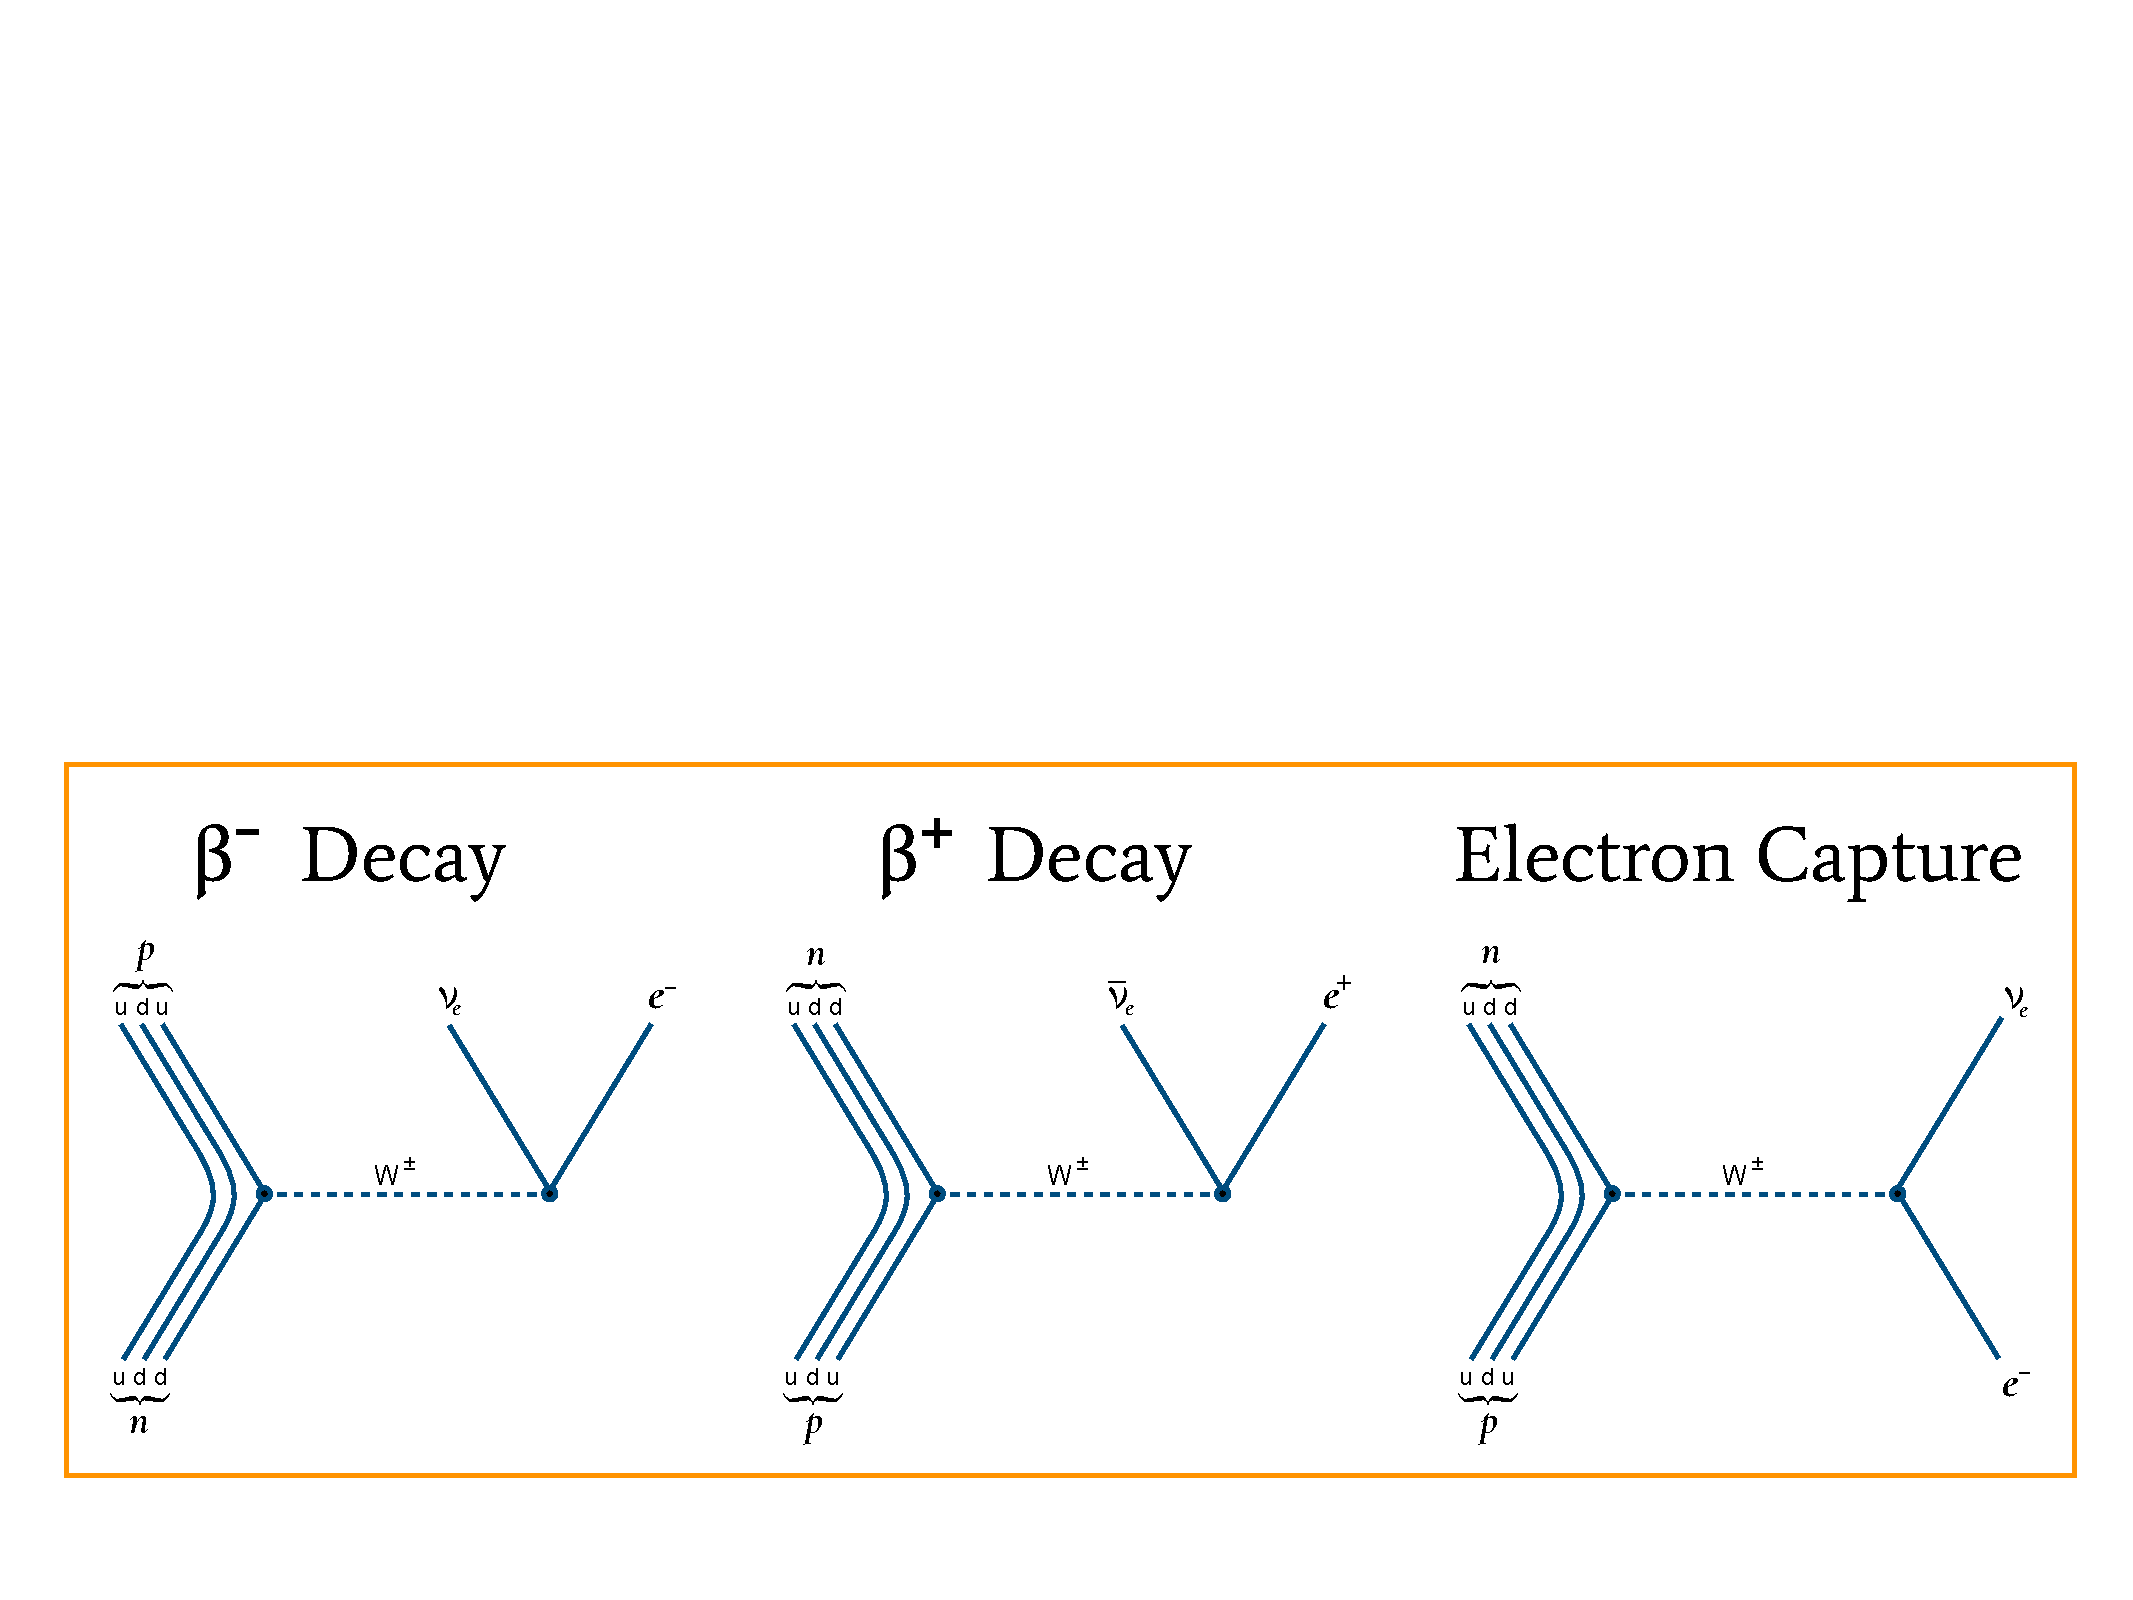
\includegraphics[width=1.0\linewidth]{Figures/BetaDecayFeynmanDiagrams.pdf}
%	\note[tag]{Fix beta decay Feynman diagram placeholder figure.}
	\caption[Beta Decay Feynman Diagrams]{Beta decay Feynman diagrams are drawn here to describe the three most common types of beta decay.  The interactions are mediated by massive $W^\pm$ bosons, resulting in an extremely limited range for the weak force.
%	 which have only a short range.
%		shown here at the nucleon(? sort of) level.    
	}	
	\label{fig:feynmandiagrams_betadecay}
\end{figure}

Energetic considerations aside, it is worthwhile to consider whether there might be any rules relating to the \emph{spin} of the nucleons before and after a decay, or the spins and angular correlations of the leptons that emerge.  Does the nucleon's spin flip during the decay process, or remain unchanged?  Are the decay products emitted preferentially in any particular direction?  Which direction are the beta and neutrino spins pointed in after they are emitted?  Angular momentum must, of course, be conserved -- but the question is \emph{how} it is to be conserved.  This question is not only at the heart of many modern precision measurements in beta decay physics, it has also been a driving force behind the development of much of our understanding of the nuclear weak force.

We must develop the tools with which these questions can be discussed.  We will begin by using Fermi's classic description of a beta decay as a transition that occurs with zero range:
\bea
\mathcal{M}_{fi} &=& G_F \int \bar{\psi}_f \, \mathcal{\hat{O}} \, \psi_i \,\textrm{d}V,
\label{eq:fermitransition}
\eea 
where $\mathcal{M}_{fi}$ is the transition matrix element between the final ($\psi_f$) and initial ($\psi_i$) states, and $G_F$ gives a measure of the strength of the coupling between states.  The integral is evaluated over phase space volume, and the operator $\mathcal{\hat{O}}$, which has yet to be determined, allows for a mathematical description of how the initial and final states must be related in order for a transition to occur.

Of course, this description represents a model of nuclear transitions which is highly simplified;  by neglecting the $W$ bosons that mediate the process and that we now know to be present, the result is a description of an interaction with zero range -- i.e., the leptons must be emitted from the exact place where the nucleon was transmuted.  Because the mediating $W$ bosons are so heavy ($m_W = 80.379(12)$\,GeV/$c^2$ ~\cite{pdg2018}), the range of the interaction is extremely limited, so the above turns out to be a very good description.  

This immediately gives rise to a rate law commonly known as Fermi's Golden Rule, 
\beq
\Gamma \;\; = \;\; \frac{1}{\tau}  \;\; = \;\; \frac{2\pi}{\hbar} \left| \mathcal{M}_{fi} \right|^2 \, \rho(E_f),
\eeq
which describes the relationship between the total transition rate $\Gamma$ (or equivalently the lifetime $\tau$), the transition matrix element $\mathcal{M}_{fi}$, and the available density of states at the final energy, $\rho(E_f)$.  We can also use this to write down the differential decay rate, 
\bea
\frac{\textrm{d}^5 \Gamma}{ \textrm{d} \Ebeta \textrm{d}\Omegahatbeta \textrm{d} \Omegahatnu } 
&=& \frac{1}{(2\pi)^5} \, \pbeta \Ebeta (E_0 - \Ebeta)^2 F_{\pm}(\Ebeta, Z^\prime) \left| \mathcal{M}_{fi} \right|^2,
\label{eq:fermidifferentialdecayrate}
\eea
where \aside{pretty sure I lost an $\hbar$.  Maybe no one will notice.  }
$\Ebeta$ and $\pbeta$ are the outgoing $\beta$'s (total) energy and momentum,
$E_0$ is the maximum possible $\beta$ energy associated with the transition, 
and $\FFpm$ is called a Fermi function (with $Z^\prime$ the proton number of the daughter), and is used to account for the electric force between the nucleus and the (charged) outgoing electron (top) or positron (bottom) \cite{Fermi1934Italian}\cite{Fermi1934German}\cite{krane}.  

With this description, the problem of characterizing the transition is reduced to determining the form of $\mathcal{\hat{O}}$.  %, or equivalently, $\mathcal{H}_{\mathrm{int}}$.  
Table~\ref{table:dirac_matrix_operators} provides a comprehensive list of all operators for which Lorentz invariance holds.  The complete transition operator $\mathcal{\hat{O}}$ must be comprised of a linear combination of these terms.  
% !TEX root = ../thesis_main.tex
%
%
%
%%%% --- * --- %%%%	
%\renewcommand{\arraystretch}{1.6}
\begin{table}[h!!!!t]
	\begin{center}
	\begin{tabular}{ l  l  l}
		\multicolumn{3}{l}{ \textbf{Lorentz Invariant Operators}}
		\\  %\hline
		\multicolumn{1}{l}{Name} 		& \multicolumn{1}{l}{ Form}   								& \multicolumn{1}{l}{Parity}   	
		\\  \hline
		%%% % %%%
		Scalar 			   				& $1$														& $+$									
		\\
		Pseudoscalar \;\;\;\;\;\;\;		& $\gamma_5$									 			& $-$				
		\\
		Vector							& $\gamma_\mu$												& $-$				
		\\
		Axial-vector					& $\gamma_\mu \gamma_5$										& $+$
		\\
		Tensor							& $\gamma_\mu \gamma_\nu - \gamma_\nu \gamma_\mu$ \;\;		& N/A									
		\\  \hline
		%%% % %%%
	\end{tabular}
	\end{center}
%	\caption[Dirac Matrix Operators]{Dirac Matrix Operators.  I need to reference this table somewhere.  Also, these are dirac matrices in 4D.  More D, different Dirac matrices.}
	\note{Ugh, I've largely just avoided talking about parity....}
	\caption[Lorentz Invariant Operators]{A complete list of operators that obey Lorentz invariance, defined in terms of Dirac $\gamma$-matrices~\cite{ben_thesis,dan_thesis}.  It can be shown that the operators listed here span the entire space, meaning that any other Lorentz invariant operator can be expressed as a sum of the above. }
%%%%%	as a result of certain symmetries in the Dirac matrices that all other Lorentz invariant operators can be reduced to these.}
	\label{table:dirac_matrix_operators}
\end{table}
%\renewcommand{\arraystretch}{1} % table:dirac_matrix_operators


An equivalent expression for Eq.~\ref{eq:fermitransition} can be written in terms of the interaction Hamiltonian $\mathcal{H}_{\mathrm{int}}$, as:
%, $\mathcal{M}_{fi}$ may be written in terms of the interaction Hamiltonian $\mathcal{H}_{\mathrm{int}}$, as 
\bea
\mathcal{M}_{fi} &=& \int \! \mathcal{H}_{\mathrm{int}} \, \textrm{d}V. 
\label{eq:transitionmatrixhamiltonian_intro}
\eea 

To obtain a full solution to the above, we will make use of the Lee-Yang interaction Hamiltonian, which provides a generalized combination of the Lorentz invariant operators and fits neatly into Eq.~\ref{eq:transitionmatrixhamiltonian_intro}~\cite{LeeYang}:
%The Lee-Yang interaction Hamiltonian is: %\aside{It's an *interaction* Hamiltonian!}
% !TEX root = ../thesis_main.tex
%
%
%%%% --- * --- %%%%	
\bea
\mathcal{H}_{\mathrm{int}} \; / \; G_F &=& (\bar{\psi}_p \psi_n)( C_S \,\bar{\psi}_e \psi_\nu + C_S^\prime \, \bar{\psi}_e \gamma_5 \psi_\nu )
%
\nonumber \\ &&
+ \: (\bar{\psi}_p \gamma_\mu \psi_n)( C_V \,\bar{\psi}_e \gamma_\mu \psi_\nu + C_V^\prime \, \bar{\psi}_e \gamma_\mu \gamma_5 \psi_\nu )
%
\nonumber \\ &&
+ \: \frac{1}{2} (\bar{\psi}_p \sigma_{\lambda \mu} \psi_n)( C_T \,\bar{\psi}_e \sigma_{\lambda \mu} \psi_\nu + C_T^\prime \, \bar{\psi}_e \sigma_{\lambda \mu} \gamma_5 \psi_\nu ) 
%
\nonumber \\ &&
- \: (\bar{\psi}_p \gamma_\mu \gamma_5 \psi_n)( C_A \,\bar{\psi}_e \gamma_\mu \gamma_5 \psi_\nu + C_A^\prime \, \bar{\psi}_e \gamma_\mu \psi_\nu )
%
\nonumber \\ &&
+ \: (\bar{\psi}_p \gamma_5 \psi_n)( C_P \,\bar{\psi}_e \gamma_5 \psi_\nu + C_P^\prime \, \bar{\psi}_e \psi_\nu ) 
%
+ \textrm{H.C.},
\label{eq:lee_yang_hamiltonian_intro} 
\eea
%%%%  \label{eq:lee_yang_hamiltonian_intro} 

Here, $C_X$ and $C_X^{\prime}$ (with $X=\{V,A,S,T,P\}$) are complex coupling constants for vector, axial, scalar, tensor, and pseudoscalar interactions, and $\psi_Y$ (with $Y=\{p,n,e,\nu\}$) are the wavefunctions for the interaction's proton, neutron, electron, and neutrino.  Operators $\gamma_5$ and $\gamma_\mu$ are Dirac gamma matrices, and $\mbox{$\sigma_{\lambda\mu} = -\frac{i}{2}(\gamma_\lambda \gamma_\mu - \gamma_\mu\gamma_\lambda )$}$.  As usual, ``H.C.'' represents the Hermitian conjugate of the previous terms within the Hamiltonian.

It can be seen from the form of the Hamiltonian that the $V,A,S,T,P$ couplings within are described as such because they \emph{behave} as vectors, axial-vectors, scalars, tensors, and pseudoscalars (respectively) under a Lorentz transform, where the Lagrangian itself must be a scalar both before and after a Lorentz transform~\cite{LeeYang}~\cite{Falkowski2021}~\cite{hong_sternberg_garcia}.

The fact that there are two coupling constants (primed and unprimed) for each type of coupling relates to the \emph{handedness} of the interaction.  Both left-handed and right-handed couplings, or a combination thereof, are \emph{a priori} possible, and the form of Eq.~\ref{eq:lee_yang_hamiltonian_intro} does not give preference to either.

While it is possible to define an interaction's handedness in a rigorous and mathematical way, the reader may gain more clarity by simply remembering the rule of thumb that a left-handed weak force 
% (which is predominantly or entirely what exists in nature) 
couples only to left-handed regular matter leptons and right-handed anti-leptons --- where the handedness of a lepton or other particle is defined by the direction of its spin relative to its direction of motion.  That description is exact in the limit where such a particle travels at the speed of light (otherwise a clever Lorentz transform can change the result), but the underlying mathematics is well defined for slower particles as well.  For neutrinos, which are so light they were long believed to be massless, the description is nearly perfect.  For electrons and positrons emitted in beta decay, which are massive but often emitted at relativistic speeds, the description is modified by inserting a factor of $v/c$ to quantify the handedness exactly.  
%is only \emph{pretty good}.  

\note{Here, we should put in Falkowski's convention to separate out the RH and LH components of things.  Or take it out completely.}

Over the years, we have collectively learned much about which simplifications to Eq.~\ref{eq:lee_yang_hamiltonian_intro} can be justified.  Typically, reference to the pseudoscalar couplings is one of the first things to be dropped, because it is suppressed at typical beta decay energies, and as such its presence would be difficult to demonstrate and have very little effect on experimental results.  
It is also now widely understood that 
the nuclear weak force involves primarily (or entirely) vector and axial vector couplings, and is primarily (or entirely) a left-handed interaction in which parity is maximally (or nearly maximally) violated.  

\note{We'll use Falkowski's convention to re-wite the Lee-Yang Hamiltonian in terms of right- and left-handed interactions.  That'll be useful later.  Sort-of.}

\note{Something about how beta decays turned out to be $(V-A)$...}

Although the physics community has largely come to a consensus 
%over the years 
on the \emph{dominant} behaviour of the nuclear weak force, there still exists a range of possible \emph{sub-dominant} behaviours that cannot be ruled out by theoretical considerations alone, and therefore must be tested experimentally.  With the weak force already so well described, searching for indications of unexpected behaviours is the domain of precision measurements.  This class of non-dominant behaviours is sometimes described as exotic physics, or with the imprecise label of physics \ac{BSM}, or even the wildly inaccurate misnomer, ``new physics''~\cite{Combs2020}\cite{GonzalesalonsoNaviliatcuncicSeverijns2019}\cite{newphysics_cirgiliano2019}\cite{newphysics_neutrinoless2015}\cite{newphysics_neutrinoless2007}\cite{newphysics_1998}\cite{newphysics_1992langacker}.  

Many types of exotic physics have, in fact, already been described by Lee and Yang's 1956 interaction Hamiltonian, which was originally motivated by the question of parity conservation within beta decay\cite{LeeYang}.  Despite the original motivations, the authors were very thorough in their description of possible interaction types.  By starting with Fermi's contact interaction model of beta decay, incorporating Gamow and Teller's selection rules, and enforcing Lorentz invariance, they arrived at a nucleon-level Hamiltonian (quarks had not been discovered yet) which accounted for \emph{all} possible coupling behaviours~\cite{GamowTeller}. 

%\note[jbn]{John vetoes the following paragraph, which admittedly is stupid.}
%In the years since, we have discovered that beta decay is mediated by $W^\pm$ bosons, which, among other things, allows for the possibility of certain transitions (ie, with different selection rules) occuring, which had been considered forbidden under the contact interaction model.  






%%%% --- * --- %%%%
\section{Our Decay}
Here, we will focus on the decay,
\bea
^{37}\textrm{K} &\rightarrow& \,^{37}\textrm{\!Ar} + \beta^{+} + \nu_e, 
\label{eq:ourdecay}
\eea
which is extremely well suited to the type of experiment to be the discussed in this thesis.  
%this and other similar experiments -- both because of its suitability 
The parent, $^{37}\textrm{K}$, is an isotope of potassium---an alkali.  Though this fact may initially seem unremarkable, it is their hydrogen-like~\aside[done, nolist]{hydrogen-like does not need quotes} single valence electron which allows alkalis to be readily trapped within a magneto-optical trap, a critical component of our experimental design (see Chapter~\ref{atomicphysics_chapter}).

A potential concern in any experiment concerned with the angular correlations resulting from one particular decay branch is the background from competing decay branches.  As can be seen in Fig.~\ref{fig:nuclearleveldiagram}, the decay of $^{37}\textrm{K}$ is dominated by a single branch which contributes nearly $98\%$ of $^{37}\textrm{K}$ decay events, and the remaining events nearly all arise from a single branch contributing around $2\%$ of the decay events.  The other branches combined account for only around $0.04\%$ of decays.  Taken all together, this means that the background events which must be accounted for are both infrequent and well understood.

\begin{figure}[h!t!b!]
	\centering
	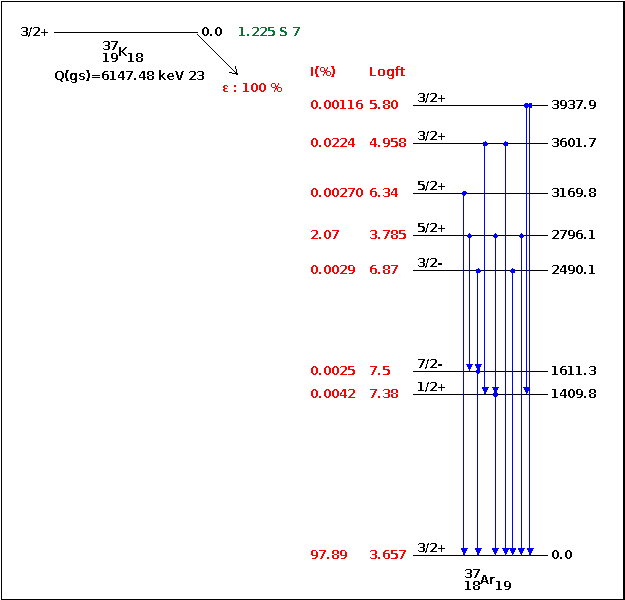
\includegraphics[width=.999\linewidth]{Figures/decayscheme_nndc.png}
	\caption[Decay Scheme for $^{37}$K]{A Decay Scheme for $^{37}$K, generated with the NuDat3 database toolset.  The $I(\%)$ column indicates the fraction of total decays which proceed to each level, and `Logft' gives a measure of the absolute decay rate\cite{krane}.  The column immediately to the right  of Logft indicates nuclear spin and parity, and the far right column is the energy relative to the ground state, in keV\cite{nucleardata2012}\cite{shidling2014}\cite{ozmetin2020}. 
	}	
	\label{fig:nuclearleveldiagram}
\end{figure}
%\FloatBarrier

\note{Re: Fig.~\ref{fig:nuclearleveldiagram}:  the picture needs needs:  title, labels on $I^\pi$ columns, label "energy" on the RH column (which kind of energy?  It's the "level energy".  
}
\note[done, nolist]{JB says Re: Fig.~\ref{fig:nuclearleveldiagram}: 
\\..\\
The caption should include that [...] log\_10(fT) [is] a measure of the absolute decay rate (ref. Krane e.g.) \cite{krane}.
the [...] column [that] has $I^\pi$ where I is spin and $\pi$ is parity [should get a label]. This should not only include Dan's thesis for a reference, but the most recent paper with the branches-- it should work to reference P.D. Shidling
et al. Phys Rev C 98 015502 (2018) \cite{shidling2014} which re-did the half-life and summarized the fT value extraction. I see no publication of your branching ratio work, so I referenced Ozmetin's DNP talk in an earlier note. \cite{ozmetin2020}
}


As in any decay, the angular correlations between the emerging daughter particles provide a rich source of information about the type of interaction that produced the decay.  
This particular decay involves a set of isobaric mirror nuclei, meaning that the nuclear wavefunctions of the parent and daughter are identical up to their isospin quantum number and corresponding electrical charge.  Because the two wavefunctions are so similar, effects to the decay from nuclear structure corrections are well understood and can be kept to a minimum, making it possible to place especially strong constraints on the size of the theoretical uncertainties associated with the decay.
%Because the higher-order standard model corrections to this decay process are well understood, it is an ideal candidate for for improving constraints on interactions beyond the standard model.  

\note[done, nolist]{no one will let you publish air quotes, ever. Have mercy on your committee, take them all out.  Use the opportunity to make sure you've defined them.
\\...\\
Here, just say isobaric mirror nuclei. You define it right there in text. It's fine to use textbook terms as long as you define them immediately.} 
\note[bluetodo]{Is it definitely true that the nuclear structure corrections are *smaller*?  Or is it just that they're better understood?}

\note{Also, 37K is a really nice isotope for this, because 
%98\% + 2\%, 
%also because it's a mirror decay, 
%also because it's an alkali.  Also-
%also, 
its big $\Abeta$ value means we have a big thing to multiply any $\bFierz$ value there might be when we construct the superratio asymmetry to eliminate systematics.}

%\missingfigure{This thing is going to need a nuclear level diagram for 37K.  Also, 37K is a really nice isotope for this, because 98\% + 2\%, also because it's a mirror decay, also because it's an alkali.  Also-also, its big $\Abeta$ value means we have a big thing to multiply any $\bFierz$ value there might be when we construct the superratio asymmetry to eliminate systematics.}







%%%% --- * --- %%%%
\section{The Physical Signature of the Fierz Interference}
%\subsection{Mathematical Description}
\label{sec:mathdescription_intro}
In this section, we consider how scalar and tensor interactions within the beta decay process might manifest as a physical observable.  As this section is, in part, intended to aid the reader in gaining a physical intuition for certain aspects of decay behaviour, only the leading order terms are described. However, the full mathematical formalism including many higher-order terms is worked out in detail within Appendix~\ref{appendix_forthepeople}.
%this section will simply provide the result directly, and use this as a starting point. 
The \ac{PDF} below provides a description of beta decay in terms of the outgoing beta's energy and direction relative to the nuclear spin, in terms of (almost) all mathematically consistent types of couplings. (Pseudoscalar couplings are neglected in this treatment, because they are relativistically suppressed at the energy scales characteristic of typical beta decays.)  This \ac{PDF} is a simplification of the one presented in the classic \ac{JTW} paper, and is accurate to leading order~\cite{jtw}\cite{jtw_coulomb}\cite{EbelFeldman1957}.  For the dominant branch of $^{37}$K decay, we have:
%This two-dimensional \ac{PDF} provides a description of beta decay in terms of the outgoing beta's energy and direction relative to the nuclear spin
%%To leading order, the probability density function from the classic \ac{JTW} paper can be used to describe beta decay in terms of the outgoing beta's energy and direction relative to the nuclear spin~\cite{jtw}\cite{jtw_coulomb}\cite{EbelFeldman1957}.  
\bea
	\textrm{d}^2 \Gamma  ( \Ebeta, \theta ) 
	&=&
	W(\Ebeta) \left[ 1 + \bFierz \frac{\m c^2}{\Ebeta} + \Abeta \, \frac{\pe c }{\Ee}\, |\vecP| \cos\theta  \right] \, \dEe \, \textrm{d} \theta , 
\nonumber \\
\label{equation:integrated_jtw_INTRODUCTION}
\eea
where $\vecP$ is the overall nuclear spin polarization, $\Ee$ and $\pe$ are the energy and momentum of the outgoing beta particle, and $\theta$ is the angle between $\vecP$ and the beta emission direction.  
As usual, $\me$ is the mass of the electron and $c$ is the speed of light.
The expression's overall energy dependence has been absorbed into the term $W(\Ebeta)$, so that
\bea
W(\Ebeta) &:=& \frac{2}{(2\pi)^3} \, \FFminus \, \xi \, \pe \Ee (E_0 - \Ee)^2,
\label{eq:overallenergydependence_intro}
\eea
where $E_0$ is the maximum possible beta energy associated with the transition.  The function $\FFminus$ is a Fermi function for outgoing positrons,
%for outgoing electrons (top) and positrons (bottom), 
with $Z^\prime$ the proton number of the daughter nucleus.  The Fermi function accounts for the force from the electric charge of the daughter nucleus and its orbital electrons acting on the outgoing electron/positron.  It is computed with the Dirac equation using various levels of approximation to describe the nuclear charge distribution and screening of that charge distribution by electrons near the nucleus.
\aside{cite:  Hayen+Severijns et.al., 2017.}

We now turn our attention to the parameters $\Abeta$ (the beta asymmetry), $\bFierz$ (the Fierz interference), and $\xi$ that are used in Eqs.~(\ref{equation:integrated_jtw_INTRODUCTION})-(\ref{eq:overallenergydependence_intro}).  These parameters are unique to the transition under consideration, but are nevertheless closely related to certain universally applicable coupling strengths.  They can be written in terms of the universally applicable complex coupling constants $C_X$ and $C_X^{\prime}$ of Eq.~(\ref{eq:lee_yang_hamiltonian_intro})
%(with $X=\{V,A,S,T,P\}$) are complex coupling constants for vector, axial, scalar, tensor, and pseudoscalar interactions
as follows: 
% !TEX root = ../thesis_main.tex
%
%
%
%%%% --- * --- %%%%	
\begin{eqnarray}
    \xi &=& 
    	|M_F|^2    \left( |C_S|^2 + |C_V|^2 + |C_S^\prime|^2 + |C_V^\prime|^2 \right) 
		\nonumber \\ && + \;\,
		|M_{GT}|^2 \left( |C_T|^2 + |C_A|^2 + |C_T^\prime|^2 + |C_A^\prime|^2 \right)
		\label{eq:jtw_xi_integrated_intro} \\
    \bFierz \, \xi &=& 
    	- \: 2 \gamma \;
		\textrm{Re}\!\left[ |M_F|^2 \left( C_S C_V^* + C_S^\prime C_V^{\prime *} \right) 
    	+ |M_{GT}|^2 \left( C_T C_A^* + C_T^{\prime} C_A^{\prime *} \right) \right] 
		\nonumber \\
    	\label{eq:jtw_bxi_integrated_intro} %\\
\end{eqnarray}
%%%	\\
\begin{eqnarray}
    \Abeta \, \xi &=& 
    	\frac{4}{5} \, |M_{GT}|^2 \left[ \textrm{Re}\!\left[ C_A C_A^{\prime *} - C_T C_T^{\prime *} \right] + \frac{\alpha Z \me c^2}{\pbeta c} \,\textrm{Im}\!\left[ C_T C_A^{\prime *} + C_T^\prime C_A^* \right] \right] 
		\nonumber \\ && + \;\, 
		2
		\left( \frac{3}{5} \right)^{\!\! 1/2} \!\!
		M_F\,M_{GT}  \left[ \phantom{\frac{1}{1}\!\!\!\!} \textrm{Re} \! \left[ C_S C_T^{\prime *} +  C_S^\prime C_T^* - C_V C_A^{\prime *} - C_V^\prime C_A^* \right] 
		\right.
		\nonumber \\ && - \;
		\left.
		\frac{\alpha Z^\prime \me c^2}{\pbeta c} \,\textrm{Im}\!\left[ C_S C_A^{\prime *} + C_S^\prime C_A^* - C_V C_T^{\prime *} -C_V^\prime C_T^* \right] \right].
	\label{eq:jtw_Abetaxi_integrated_intro}
\end{eqnarray}
%
%\aside{I'm missing factors of $c$ in this.  Probably put them in.  ...naw, it looks fine.}
%

In the above expressions, $M_F$ and $M_{GT}$ are the Fermi (vector coupling) and Gamow-Teller (axial coupling) matrix elements unique to a particular transition,~\aside[note]{See Appendix~\ref{sec:jtw_formalism}, I guess?} and 
\\
\mbox{$\gamma := \left( 1-\alpha^2 Z^{\prime 2} \right)^{1/2} \approx 1$}, using fine structure constant $\alpha$.
%\note[note,nolist]{}
\aside[note]{I've specialized to the 98\% branch already.  Did I say so?}

The expressions above have many free parameters, and some simplifications and assumptions must be made before any experimental measurement can be interpreted in a physically meaningful way.  
%a physically meaningful measurement can be made.  
We note that each type of interaction $X$ (for $X=\{V,A,S,T\}$) is described by \emph{two} complex coupling constants, $C_X$ and $C_X^\prime$;  this extra degree of freedom is necessary in order to describe couplings to both left-handed and right-handed helicity leptons.
~\aside{Is it definitely helicity?  Or do I mean chirality?  I think helicity is right.  probably.}
In practice, we already know that the weak force couples (almost) entirely to left-handed electrons and right-handed positrons.  Separately, we know that the interaction proceeds (almost) entirely by vector and axial couplings.  Taken together, this suggests that neutrinos and anti-neutrinos, as leptons, must (predominantly) follow the same helicity selection rules that apply to electrons and positrons.  This is because, \emph{e.g.}, a decay mediated by either scalar or tensor couplings would produce two outgoing leptons/anti-leptons of the \emph{same} helicity.  

It is this subtlety which gives rise to the energy dependence ($\me c^2 / \Ee $) by which $\bFierz$ is multiplied in Eq.~(\ref{equation:integrated_jtw_INTRODUCTION}).  
%--- it is fundamentally an \emph{interference} term between the interactions of standard model physics with an unknown exotic physics term.  
That is, if we have restricted ourselves to interactions involving right-handed anti-neutrinos travelling at the speed of light, then the scalar or tensor components of this interaction, if present, must also couple to right-handed helicity electrons.  The lower the energy of the outgoing electron, the greater the fraction of available phase space in which the electron appears to be right-handed from the reference frame of the mediating $W$-boson.  In other words, this term describes a mechanism by which scalar and tensor couplings can effectively compete with the expected vector and axial couplings~\cite{hong_sternberg_garcia}\cite{Greiner2009}.
%;  this is why $\bFierz$ is described as an \emph{interference} term~\cite{hong_sternberg_garcia}\cite{Greiner2009}.
% effectively competing with the expected vector and axial couplings.  

As a practical matter, the ($\me c^2 / \Ee $) dependence of the Fierz term suggests that $\bFierz$ is best measured by a relatively low-energy experiment (such as the one described here) in order to maximize sensitivity;  a high-energy experiment would have trouble constraining it.


\note{somewhere:  point out that $\bFierz$ is linear in BSM.  other observables are quadratic.  So this way is best for small S, T couplings.}
%\note[note,nolist]{}
\note[tag]{Needs:  
\\
%* also, we describe it in that order [despite the fact that we're actually (experimentally?) limited to the one helicity of electrons but we have no experimental limits on neutrino helicity really...], because with massive electrons you can boost to a frame with opposite helicity.  `Massless' neutrinos can't do that.  So you get a factor of electron mass in there.
%
%* citations for Ran Hong and Greiner2009.  They go here.  --> done!
%\\
* ...Also, it arises from the Dirac spinor term?
%\\
%* Practically, it means we're sensitive to this and high energy is not.
}

We will henceforth take $C_X = C_X^\prime$, which is equivalent to a requirement that all couplings are left-handed.  We define a set of purely left-handed couplings:
\bea
g_V &=& \frac{1}{\sqrt{2}}  \, (C_V + C_V^\prime )  %\;\; = \;\; +\, 1.0
\label{eq:gV_def}
\\
g_A &=& \frac{-1}{\sqrt{2}} \, (C_A + C_A^\prime )  %\;\; \approx \;\; +\, 0.91210
\label{eq:gA_def}
\\
g_S &=& \frac{1}{\sqrt{2}} \, (C_S + C_S^\prime ) 
\label{eq:gS_def}
\\
g_T &=& \frac{-1}{\sqrt{2}} \, (C_T + C_T^\prime).
\label{eq:gT_def}
\eea
Furthermore, we will also require going forward that all $C_X$ must be \emph{real};  this is equivalent to requiring that the interactions obey time-reversal invariance. 
%\note[note,nolist]{}
%If one assumes the standard model holds, $\Abeta$, $\bFierz$, and $\xi$ can be written in terms of a greatly simplified set of parameters.  
We also introduce $\rho$, the ratio of Gamow-Teller and Fermi couplings:  %$\rho$ is unique to a particular transition, and must be measured experimentally.  
\bea
\rho &:=& \frac{C_A M_{GT}}{C_V M_F}  \;\; = \;\; \frac{- g_A M_{GT}}{g_V M_F}.
\label{eq:definerho_intro}
\eea
The value of $\rho$ is unique to a particular transition, and must be extracted experimentally (see Sec.~\ref{sec:extractinglambda}).
~\aside[note]{See Appendix~\ref{sec:combo_formalism} for a discussion of the relationship between parameters $C_X$ and $g_X$.  I guess.}  

Using the above notation and the simplifying assumptions that give rise it, and dropping terms of order (small)$^2$ or higher, it is possible to re-write Eqs.~(\ref{eq:jtw_xi_integrated_intro})-(\ref{eq:jtw_Abetaxi_integrated_intro}) as:

\bea
\xi &=& 2 \,\, C_V^2 \, | M_F |^2 \left( 1 + \rho^2 \right)
\label{eq:xiwithrho_intro} 
\\
\bFierz &=& \frac{-2\gamma}{1 + \rho^2} \left( \frac{g_S}{g_V} + \rho^2 \frac{g_T}{g_A} \right). 
\label{bFierzwithlambda}
\\
\Abeta &=& \frac{\frac{2}{5} \rho^2 - 2 \rho \sqrt{\frac{3}{5}}  }{1 + \rho^2},
\label{eq:Awithrho_intro}
\eea
where $\bFierz$ reduces to 0 in the standard model limit where $g_S = g_T = 0$.  Notably, $\bFierz$ is the only term within our beta decay \ac{PDF} which includes (small) exotic couplings at the \emph{linear} order;  $g_S$ and $g_T$ arise only at quadratic order within the other terms, and thus have been dropped from Eqs.~(\ref{eq:xiwithrho_intro}) and (\ref{eq:Awithrho_intro}) above.



\note[note,nolist]{}
\note[note,nolist]{}

%%%%%%%\note[done,nolist]{JB:  I don't see where you mention the experimentally produced $M_F/M_{GT}$ that goes into the calculation for $\Abeta$.  You have the references.  You could at least say that Eq. 1.11 combined with the measured ft value produces $\lambda$, which in turn produces $\Abeta$.}  
%%%Then, specializing to the 98\% branch of $^{37}$K decay, and given the expected behaviour of the standard model,
%%%%\aside[tag]{We've specialized to 37K without telling anyone here!!!  Can't do that unless we say so.} 
%%%we can express $\xi$, $\bFierz$, and $\Abeta$ as:
%%%\bea
%%%\xi &=& 2 \,\, C_V^2 \, | M_F |^2 \left( 1 + \rho^2 \right)
%%%%\label{eq:xiwithrho_intro} 
%%%\\
%%%\bFierz &=& 0 
%%%%\label{bFierzwithrho_intro}
%%%\\
%%%\Abeta &=& \frac{\frac{2}{5} \rho^2 - 2 \rho \sqrt{\frac{3}{5}}  }{1 + \rho^2}.
%%%%\label{eq:Awithrho_intro}
%%%\eea
%%%
%%%%\note{The formalism that gave rise to these expressions is missing some things...}
%%%
%%%%\note{some citations:\\
%%%%Dan's $\Bnu$:  \cite{dan_Bnu}.
%%%%P.Shidling's $^{37}$K halflife:  \cite{shidling2014} }

\note[note]{
Deleted paragraph:
\\...\\
Because the nucleus is significantly more massive than either of the other two outgoing particles, the great majority of the released kinetic energy is distributed between the leptons, while the nucleus receives only a tiny fraction of the total.  This feature lends itself to an approximation, as above, in which the energy of the recoiling nucleus (the ``recoil'') is neglected entirely, and the decay may be described only in terms of the momenta of the outgoing positron(electron) and neutrino(anti-neutrino).  
%, as in the description from \ac(JTW)~\cite{jtw}~\cite{jtw_coulomb}.  
The terms that have been neglected in this treatment are sometimes called recoil-order corrections.
}

%In order to proceed with a measurement, we must find an equation to describe the probability of beta decay events with any given distribution of energy and momenta among the daughter particles, as a function of the strength of the specific couplings of interest to us.  To do this, two sets of formalisms are combined -- the older formalism of JTW, %~\cite{jtw},~\cite{jtw_coulomb}, 
%which describes the effects of all types of Standard Model and exotic couplings of interest to us here, but which truncates its expression at first order in the (small) parameter of transferred nuclear recoil energy, and a newer formalism from Holstein~\cite{holstein}, which includes terms up to several orders higher in recoil energy, but which does not include any description of the exotic couplings of particular interest to us.  


%%%Within this work, we are particularly interested in the $\bFierz$ parameter.  Though it is identically zero under the standard model, it is quite sensitive to certain \ac{BSM} physics.  In particular, it describes (small) left-handed scalar and tensor couplings at \emph{linear} order, while these \ac{BSM} parameters only enter at the quadratic order in the case of $\xi$ and $\Abeta$.  


%%In particular, in terms of the left-handed scalar and tensor couplings $g_S$ and $g_T$, $\bFierz$ has the form 
%%\bea
%%\bFierz &=& \frac{-2\gamma}{1 + \rho^2} \left( \frac{g_S}{g_V} + \rho^2 \frac{g_T}{g_A} \right). 
%%%\label{bFierzwithlambda}
%%\eea
%%%Here $\gamma := \left( 1-\alpha^2 Z^{\prime 2} \right)^{1/2} \approx 1$, where $Z^\prime$ is the atomic number of the daughter, and as usual $\alpha$ is the fine structure constant. 
%It is clear that Eq.~\ref{bFierzwithlambda} reduces to 0 in the standard model limit where $g_S = g_T = 0$.
%$\gamma \approx 1$ is defined as in Appendix~\ref{sec:jtw_formalism}, and\



%
\note[done,nolist]{This is where Juliette thinks I need more info about Abeta and bFierz.  
\\
``On the bottom of page 14 she lists relevant quantities (including bFierz itself) but sends the reader to an appendix rather than defining them here.''}

\note[done,nolist]{John says:  My suggested remedy:
\\
First write $b_F$ in JTW terms of $C_S$, $C_S$', $C_T$, $C_T$' and the $C_V$'s.
\\
say
`, and in notation that makes clear the lepton helicity dependence of the unknown physics,' 
\\
include your present equation in terms of $g_S$ , $g_T$.
\\ ... \\
``We have defined $g_S$, $g_T$ fully in Appendix~\ref{appendix_forthepeople}, but here summarize the main reason for this notation. The Fierz interference is between a SM term and an unknown physics term. The SM weak interaction couples to left-handed neutrinos and right-handed electrons, yet all scalar and tensor terms couple to
same-handed leptons only. So when restricting ourselves to scalars and tensors
coupling to left-handed neutrinos, they must be coupling to left-handed electrons as well. This is why the Fierz term is suppressed by the spinor factor m/E in equation 1.9 (a derivation without Dirac formalism is in (cite Hong et al. 2017 Ref. 48) the full derivation is in Greiner2009.''
\\...\\
then you really should keep going qualitatively
\\...\\
``This m/E factor is further heuristically related to
the fact that a massive particle has helicity depending on frame-- one can always boost to a frame moving faster than the particle, thus observing it rotating the same way but moving the opposite way and thus with the opposite helicity. These effects are greatly suppressed in high-energy physics, and are less suppressed in nuclear beta decay where electron energies can be similar to their mass.''
\\...\\
W. Greiner and B. M\"uller, Gauge Theory of Weak Interactions, Springer, 4th ed. 2009.
}
\note[done,nolist]{JB on JM's complaint:  
\\
Juliette has done you and us a real service here.
You write down the Fierz term in helicity terms previously undefined.
You list that in an Appendix, ok, but odd, so JM objects.
\\...\\
Her uneasiness is spot on: you state something about the helicity notation, yes, but although we've agreed you shouldn't do the actual Fierz calculation (which is in Ian's SNIT notes, and in the Greiner and Mueller weak interactions book where Albert cites it in his lectures),
unfortunately, but fortunately because it's easy to fix,
\\...\\
it looks to me like you've \textbf{neglected both the main reason for the $m/E$} (worked out without Dirac matrices in Hong's paper with Alejandro, which you cite but not for this reason-- you should not do this, but you should cite it)
and, I think?, \textbf{its practical implications} (we're sensitive to it and high-energy is not). 
%Leah Broussard covered this last point in a neutron beta decay talk at Winnipeg awhile back (we would be listing her as a possible external but universities insist in more supervisory experience).
}




%%%% --- * --- %%%%
%%%% --- * --- %%%%
%%%% --- * --- %%%%
\section{The Superratio}
\label{signature_chapter}
In considering Eqs.~(\ref{equation:integrated_jtw_INTRODUCTION})-(\ref{eq:overallenergydependence_intro}), we see that the $\bFierz$ term includes an explicit energy dependence.  From this, it seems natural to conclude that the shape of the beta energy spectrum can be used to measure the value of $\bFierz$.  This assertion is correct as far as it goes --- but a direct measurement of the complete energy spectrum is arguably not the best way to approach the matter.  In fact, it is possible to extract a much clearer signal to measure both $\Abeta$ and $\bFierz$ by making some clever choices in how our data should be processed.  
To see this, it is helpful to consider the $\Abeta$ term within Eq.~(\ref{equation:integrated_jtw_INTRODUCTION}), which carries an explicit angular dependence as well as its own explicit energy dependence.  

Though a judicious choice of detector placements, it is possible to measure the beta energy spectrum at its angular extrema, with $\cos\theta \approx \pm 1$ (recall that $\theta$ is defined to be the angle between direction of nuclear polarization and beta emission).  
\aside{Of course, the $\Abeta$ term vanishes for decays from spin-zero nuclei.}  
With differing contributions to each angle-selected beta spectrum from the $\Abeta$ term (and no other angular dependence), it is clear that any nonzero $\bFierz$ term must provide a different \emph{fractional} contribution to the full spectrum as a function of angle.
%\aside{Recall that this is angle between polarization and emission.}  

One way to quantify this fractional difference might be to take a simple ratio of the two spectra, evaluated at each energy bin --- however the effect of a non-zero $\bFierz$ term would be quite small in comparison with the overarching angular dependence of $\Abeta$.  Indeed, with the observed beta spectra explicitly selected according to emission angle, it makes little sense to attempt to extract a measurement of $\bFierz$ without a simultaneous measurement of $\Abeta$.  With this caveat kept in mind, we will now work towards finding an expression for $\Abeta$ in terms of experimental observables, with the understanding that an expression for $\bFierz$ will follow naturally.  
%--- however we will soon see that we can do better than this.  

We will approach the problem by first separating beta energy spectral data into categories relating to the angular dependence of an individual event with respect to the direction of nuclear spin.  % (which parameterizes the $\Abeta$ observable).  
If, as in our case, these sets of data can be further subdivided into categories that can be expected to measure similar physical behaviours, but which may have differing systematic effects, it is possible to force many of these these systematic effects to cancel out at leading order, as we will soon see.  

%For example, in our case, the nuclear polarization is flipped periodically within a (mostly) symmetric apparatus, with beta detectors above and below along the axis of polarization.  
%
For example, within the \ac{TRINAT} experimental setup, the polarization is flipped periodically between two states (+/-), within a (mostly) symmetric apparatus.  Two similar beta detectors (T/B) are positioned opposite one another along the vertical axis of polarization at the top and bottom of the experimental chamber (see Chapter~\ref{experimental_chapter}).  Then, with two detectors and two polarization states, we can describe four different experimental count rates based on Eq.~(\ref{equation:integrated_jtw_INTRODUCTION}).  Neglecting scattering effects, we have:
\bea
\!\! \!\!
r_{\mathrm T+}(\Ebeta) &=& W(\Ebeta)\, \varepsilon_{\mathrm T}(\Ebeta)\, \Omega_{\mathrm T} \, N_+ \left[1 + \bFierz \frac{\m c^2}{\Ebeta}  + \Abeta \, \frac{v}{c} |\vecP_{\bm{+}}| \langle \cos\theta \rangle_{\mathrm T+} \right] \;\;\;  \label{eq:r1} \\
\!\! \!\!
r_{\mathrm B+}(\Ebeta) &=& W(\Ebeta)\, \varepsilon_{\mathrm B}(\Ebeta)\, \Omega_{\mathrm B} \, N_+ \left[1 + \bFierz \frac{\m c^2}{\Ebeta}  + \Abeta \, \frac{v}{c} |\vecP_{\bm{+}}| \langle \cos\theta \rangle_{\mathrm B+} \right] \;\;\;  \label{eq:r2}\\
\!\! \!\!
r_{\mathrm T-}(\Ebeta) &=& W(\Ebeta)\, \varepsilon_{\mathrm T}(\Ebeta)\, \Omega_{\mathrm T} \, N_- \left[1 + \bFierz \frac{\m c^2}{\Ebeta}  + \Abeta \, \frac{v}{c} |\vecP_{\bm{-}}| \langle \cos\theta \rangle_{\mathrm T-} \right] \;\;\;  \label{eq:r3}\\
\!\! \!\!
r_{\mathrm B-}(\Ebeta) &=& W(\Ebeta)\, \varepsilon_{\mathrm B}(\Ebeta)\, \Omega_{\mathrm B} \, N_- \left[1 + \bFierz \frac{\m c^2}{\Ebeta}  + \Abeta \, \frac{v}{c} |\vecP_{\bm{-}}| \langle \cos\theta \rangle_{\mathrm B-} \right], \;\;\; \label{eq:r4}
\eea
%
where the $\varepsilon_{\mathrm T / \mathrm B}(\Ebeta)$ are the (top/bottom) detector efficiencies, $\Omega_{\mathrm T / \mathrm B}$ are the fractional solid angles from the trap position to the (top/bottom) detector from the trap position, $N_{+/-}$ are the number of atoms trapped in each (+/-) polarization state, and $|\vecP_{\bm{+/-}}|$ are the magnitudes of the polarization along the detector axis for each polarization state.  $\langle \cos\theta \rangle_{\mathrm T/ \mathrm B, +/-} $ is the average of $\cos\theta$ for \emph{observed} outgoing betas, 
%(\emph{i.e.}, observed in a detector with $\cos\theta \approx \pm 1$ in the present experiment), 
for each detector and polarization state combination.  This latter term is approximately $\pm 1$ as a result of our detector geometry, but contains important sign information.  

\note[note, nolist]{}
For a pointlike trap in the center of the chamber, 103.484 mm from either (DSSSD) detector,~\aside{Does this even agree with whatever I wrote about the geometry in the other section?} each of which is taken to be circular with a radius of 15.5 mm, we find that $\langle | \cos\theta | \rangle_{\mathrm T/ \mathrm B, +/-} \approx 0.994484$, and is the same for all four cases.
\aside{Not quite true.  Some strips are missing.}
% (or for $r=15.0$\,mm, we find that $\langle | \cos\theta | \rangle_{\mathrm T/ \mathrm B, +/-} \approx 0.994829$). 
\aside{This is only true if we neglect (back-)scatter.  This is not actually a good approximation.  But we have pretty good simulations to give us the real numbers, anyway. } Note that a horizontally displaced trap will decrease the magnitude of $\langle | \cos\theta | \rangle $, but as it is an expectation value of an absolute value, all four will remain equal to one another.  In the case of a vertically displaced trap, these four values will no longer all be equal, however it will still be the case that $\langle | \cos\theta | \rangle_{\mathrm T +} = \langle | \cos\theta | \rangle_{\mathrm T -}$, and $\langle | \cos\theta | \rangle_{\mathrm B+} = \langle | \cos\theta | \rangle_{\mathrm B -}$.  \aside{Is that definitely true, or is it only true to lowest order?}
\note[note, nolist]{}

%\note[note,nolist]{}

Recalling the form of the overall energy dependence $W(\Ebeta)$ from Eq.~(\ref{eq:overallenergydependence_intro}), we note that the presence of the Fermi function $\FFminus$ at any reasonable level of approximation makes $W(\Ebeta)$ integrable only by numerical methods.  As a result, there is little that could be changed to make the expression more difficult to work with, so we can safely take $W(\Ebeta)$ to be an arbitrary function.  Therefore, for the remainder of this section, we will take $W(\Ebeta)$ to implicitly include the small corrections to overall energy dependence that arise from e.g.\! recoil-order corrections, as described by Holstein~\cite{holstein}.


These four beta spectra can be used to construct the so-called superratio and superratio asymmetry, both of which have some very useful properties.  The latter of these is the measure that will eventually be used to extract the values of $\Abeta$ and $\bFierz$.   

We define the superratio, $s$, as:
\bea
s \;\;=\;\; s(\Ebeta) \;\;:=\;\; \frac{ r_{\mathrm T-}\, r_{\mathrm B+} }{ r_{\mathrm T+}\, r_{\mathrm B-} } , 
\eea
and the superratio asymmetry, $A_{\mathrm{super}}$, as:
\bea
A_{\mathrm{super}} \;\;=\;\; A_{\mathrm{super}}(\Ebeta) &:=& \frac{1-\sqrt{s}}{1+\sqrt{s}} 
\\
&=& \frac{ \sqrt{r_{\mathrm T+}\, r_{\mathrm B-} \phantom{ (\!\!\!\!\!) } }\; -\, \sqrt{ r_{\mathrm T-}\, r_{\mathrm B+}\phantom{ (\!\!\!\!\!) }} }{ \sqrt{r_{\mathrm T+}\, r_{\mathrm B-}\phantom{ (\!\!\!\!\!) }} \;+\, \sqrt{r_{\mathrm T-}\, r_{\mathrm B+} \phantom{ (\!\!\!\!\!) }} }.
\eea
%
\note[oldnote, nolist]{We used to have:  $s := \frac{ r_{\mathrm T+}\, r_{\mathrm B-} }{ r_{\mathrm T-}\, r_{\mathrm B+} }$, and the $A_{\mathrm{super}}$ that follows.  But that's wrong.  :(   Need $s > 1$ to get the right result.}

This is explicitly an experimental quantity that is measured directly by the above combination of count rates, however it is obvious that it reduces, under appropriate limits, to be equivalent to a naive asymmetry.  In particular, if we require that the physical conditions and relative detector positions and sensitivities are identical when the polarization is flipped, then we have $r_{\mathrm T+}(\Ebeta) = r_{\mathrm B-}(\Ebeta)$, $r_{\mathrm T-}(\Ebeta) = r_{\mathrm B+}(\Ebeta)$, and $|\vecP_{\bm{+}}| = |\vecP_{\bm{-}}|$.
%
With these simplifying assumptions, the superratio asymmetry quickly reduces into a more intuitive quantity that we might use for a measurement with only a single polarization state, e.g.,  
%%\bea
%%A_{\mathrm{super}} &\rightarrow& \frac{ r_{\mathrm T+}\, - \,r_{\mathrm B+} }{r_{\mathrm T+}\, +\, r_{\mathrm B+} } 
%%\;\;\; \rightarrow \;\;\; \Abeta \frac{v}{c} |\vecP| . 
%%\label{eq:singlepol_asymmetry}
%%\eea
%\bea
%A_{\mathrm{super}} &\rightarrow& \frac{ r_{\mathrm T+}\, - \,r_{\mathrm B+} }{r_{\mathrm T+}\, +\, r_{\mathrm B+} } 
%\;\;\; \rightarrow \;\;\; \Abeta \frac{v}{c} |\vecP_{\bm{+}}| \: |\langle \cos\theta \rangle| . 
%\label{eq:singlepol_asymmetry}
%\eea
\bea
A_{\mathrm{super}} &\rightarrow& \frac{ r_{\mathrm T+}\, - \,r_{\mathrm B+} }{r_{\mathrm T+}\, +\, r_{\mathrm B+} } 
\;\;\; \xrightarrow[\bFierz = 0]{} \;\;\; \Abeta \frac{v}{c} |\vecP_{\bm{+}}| \: \langle | \cos\theta | \rangle . 
\label{eq:singlepol_asymmetry}
\eea
%\note{Assumes $\bFierz=0$.  Or, rather, we can only interpret it as $\Abeta$ if $\bFierz=0$.  }

The superratio, and superratio asymmetry, has been used for precision beta decay measurements in the past to measure the neutron's beta asymmetry\cite{UCNA_first_superratio}, and our own collaboration has also used it to measure the beta asymmetry in $^{37}$K~\cite{ben_Abeta}.  More recently, it has been used to measure the neutron's Fierz interference term~\cite{UCNAfierz2020}\cite{Saul2020} as well, with notably more impressive results than using the earlier `supersum' data combination method~\cite{UCNA_first_Fierz}.  


%%%\note{}
%%%In the case of the present experiment, we note that $|\vec{P}_+| = |\vec{P}_-|$ is correct to a high degree of precision.
%%%\note{}



While Eq.~\ref{eq:singlepol_asymmetry} is conceptually encouraging, the assumptions that gave rise to it are too simplifying.  
%
Fortunately, as we'll soon see, the key to the effectiveness of the superratio technique is that many systematic effects can be made to cancel at the leading order, at the cost of some statistical resolving power.  
%
We will introduce some less restrictive assumptions for what follows, along with shorthand notation for improved readability (and to make it obvious which quantities are to be considered small).  First, we require that the magnitude of the polarization vector is the same for both polarization states (within the present experiment, $|\vecP_{\bm +}| = |\vecP_{\bm -}|$ is correct to a high degree of precision), and also that the average of the magnitude of $\cos\theta$ for a given detector does not change when the polarization is flipped (equivalent to a requirement that the trap position doesn't change when the polarization is flipped).  Then: 
\bea
P &:=& |\vecP_{\bm +}| = |\vecP_{\bm -}|  \\
\langle |\cos\theta | \rangle_T &:=& \langle |\cos\theta | \rangle_{\mathrm T+} \, = \, \langle |\cos\theta | \rangle_{\mathrm T-} \\
\langle |\cos\theta | \rangle_B &:=& \langle |\cos\theta | \rangle_{\mathrm B+} \, = \, \langle |\cos\theta | \rangle_{\mathrm B-},
\eea
and we can further define
\bea
c &=& \,\,\,\,\, \langle | \cos\theta | \rangle :=  \frac{1}{2} \left( \phantom{2_2^2}\!\!\!\! \langle |\cos\theta | \rangle_T + \langle |\cos\theta | \rangle_B \, \right) \\
\Delta c &=& \Delta \langle | \cos\theta | \rangle := \frac{1}{2} \left( \phantom{2_2^2}\!\!\!\! \langle |\cos\theta | \rangle_T - \langle |\cos\theta | \rangle_B \, \right)
\eea
and 
\bea
\tilde{A} &=\;\; \tilde{A}(\Ebeta) &:=\;\; A_\beta \frac{v}{c} \\ 
\tilde{b} &=\;\; \tilde{b}(\Ebeta) &:=\;\;  \bFierz \frac{mc^2}{\Ebeta}, \\
\tilde{r} &=\;\; \tilde{r}(\Ebeta) &:=\;\; 1+\tilde{b}. 
\eea

With this new set of variables defined, we can re-write Eqs.~(\ref{eq:r1}-\ref{eq:r4}) as
\bea
r_{\mathrm T+}(\Ebeta) &=& W(\Ebeta)\, \varepsilon_{\mathrm T}(\Ebeta)\, \Omega_{\mathrm T}\, N_+ \left[\tilde{r}  \,+\, \tilde{A} P \left( \phantom{2_2^2}\!\!\!\! c + \Delta c \, \right) \right] \\
r_{\mathrm B+}(\Ebeta) &=& W(\Ebeta)\, \varepsilon_{\mathrm B}(\Ebeta)\, \Omega_{\mathrm B}\, N_+ \left[\tilde{r}  \,-\, \tilde{A} P \left( \phantom{2_2^2}\!\!\!\! c - \Delta c \, \right) \right] \\
r_{\mathrm T-}(\Ebeta) &=& W(\Ebeta)\, \varepsilon_{\mathrm T}(\Ebeta)\, \Omega_{\mathrm T}\, N_- \left[\tilde{r}  \,-\, \tilde{A} P \left( \phantom{2_2^2}\!\!\!\! c + \Delta c \, \right) \right] \\
r_{\mathrm B-}(\Ebeta) &=& W(\Ebeta)\, \varepsilon_{\mathrm B}(\Ebeta)\, \Omega_{\mathrm B}\, N_- \left[\tilde{r}  \,+\, \tilde{A} P \left( \phantom{2_2^2}\!\!\!\! c - \Delta c \, \right) \right], 
\eea
and the superratio becomes
\bea
s 
&=& 
\frac{ 
\left(
\tilde{r} + \tilde{A} P c \right)^2 -  \left( \phantom{\tilde{2}_2^2}\!\!\!\!\! \Delta c \right)^2 
}{ 
\left(
\tilde{r} - \tilde{A} P c \right)^2 -  \left( \phantom{\tilde{2}_2^2}\!\!\!\!\! \Delta c \right)^2 
} 
\eea
where all factors of $W(\Ebeta)$, $\varepsilon_{\mathrm T/B}(\Ebeta)$, $\Omega_{\mathrm T/B}$, and $N_{+/-}$ have been cancelled out entirely.  

For simplicity we take $\Delta c = 0$ in what follows.  Although this is not strictly accurate within the present experiment, this assumption greatly simplifies the expressions that follow.  Then, absent other corrections (\emph{e.g.} backscattering, unpolarized background, ...), it is clear that if $\tilde{b} = 0$ as in the Standard Model, %it follows that 
\bea
A_{\mathrm{super}} &=\;\; \tilde{A} P c &=\;\; \Abeta \, \frac{v}{c} \, |\vec{P}| \, \langle | \cos\theta | \rangle
\eea

In the case where $\tilde{b} \neq 0$, we find that 
\bea
A_{\mathrm{super}} &=& \frac{\tilde{A} P c}{1+\tilde{b}} \\
&\approx&  \tilde{A} P c \, (1 - \tilde{b} + {\tilde{b}}^2),
\eea
where we have utilized the assumption that $\tilde{b} \ll 1$.
Thus, to leading order in terms of $\tilde{b}$, 
\bea
A_{\mathrm{super}} &\approx& \Abeta \, \frac{v}{c} \, |\vec{P}| \, \langle | \cos\theta | \rangle \left( 1 - \bFierz \frac{mc^2}{\Ebeta} \right).
\eea


In addition to eliminating systematic effects, the superratio asymmetry also provides an enhanced signal to be evaluated, as can be seen in Fig.~\ref{fig:FierzSignature}.  The price for this clear signal and reduction in systematics is, unfortunately, a decrease in overall statistical resolving power.  Given the difficulty of controlling many of the cancelled systematics, this can potentially be a very good trade-off.  

\begin{figure}[h!!tb]
	\centering
	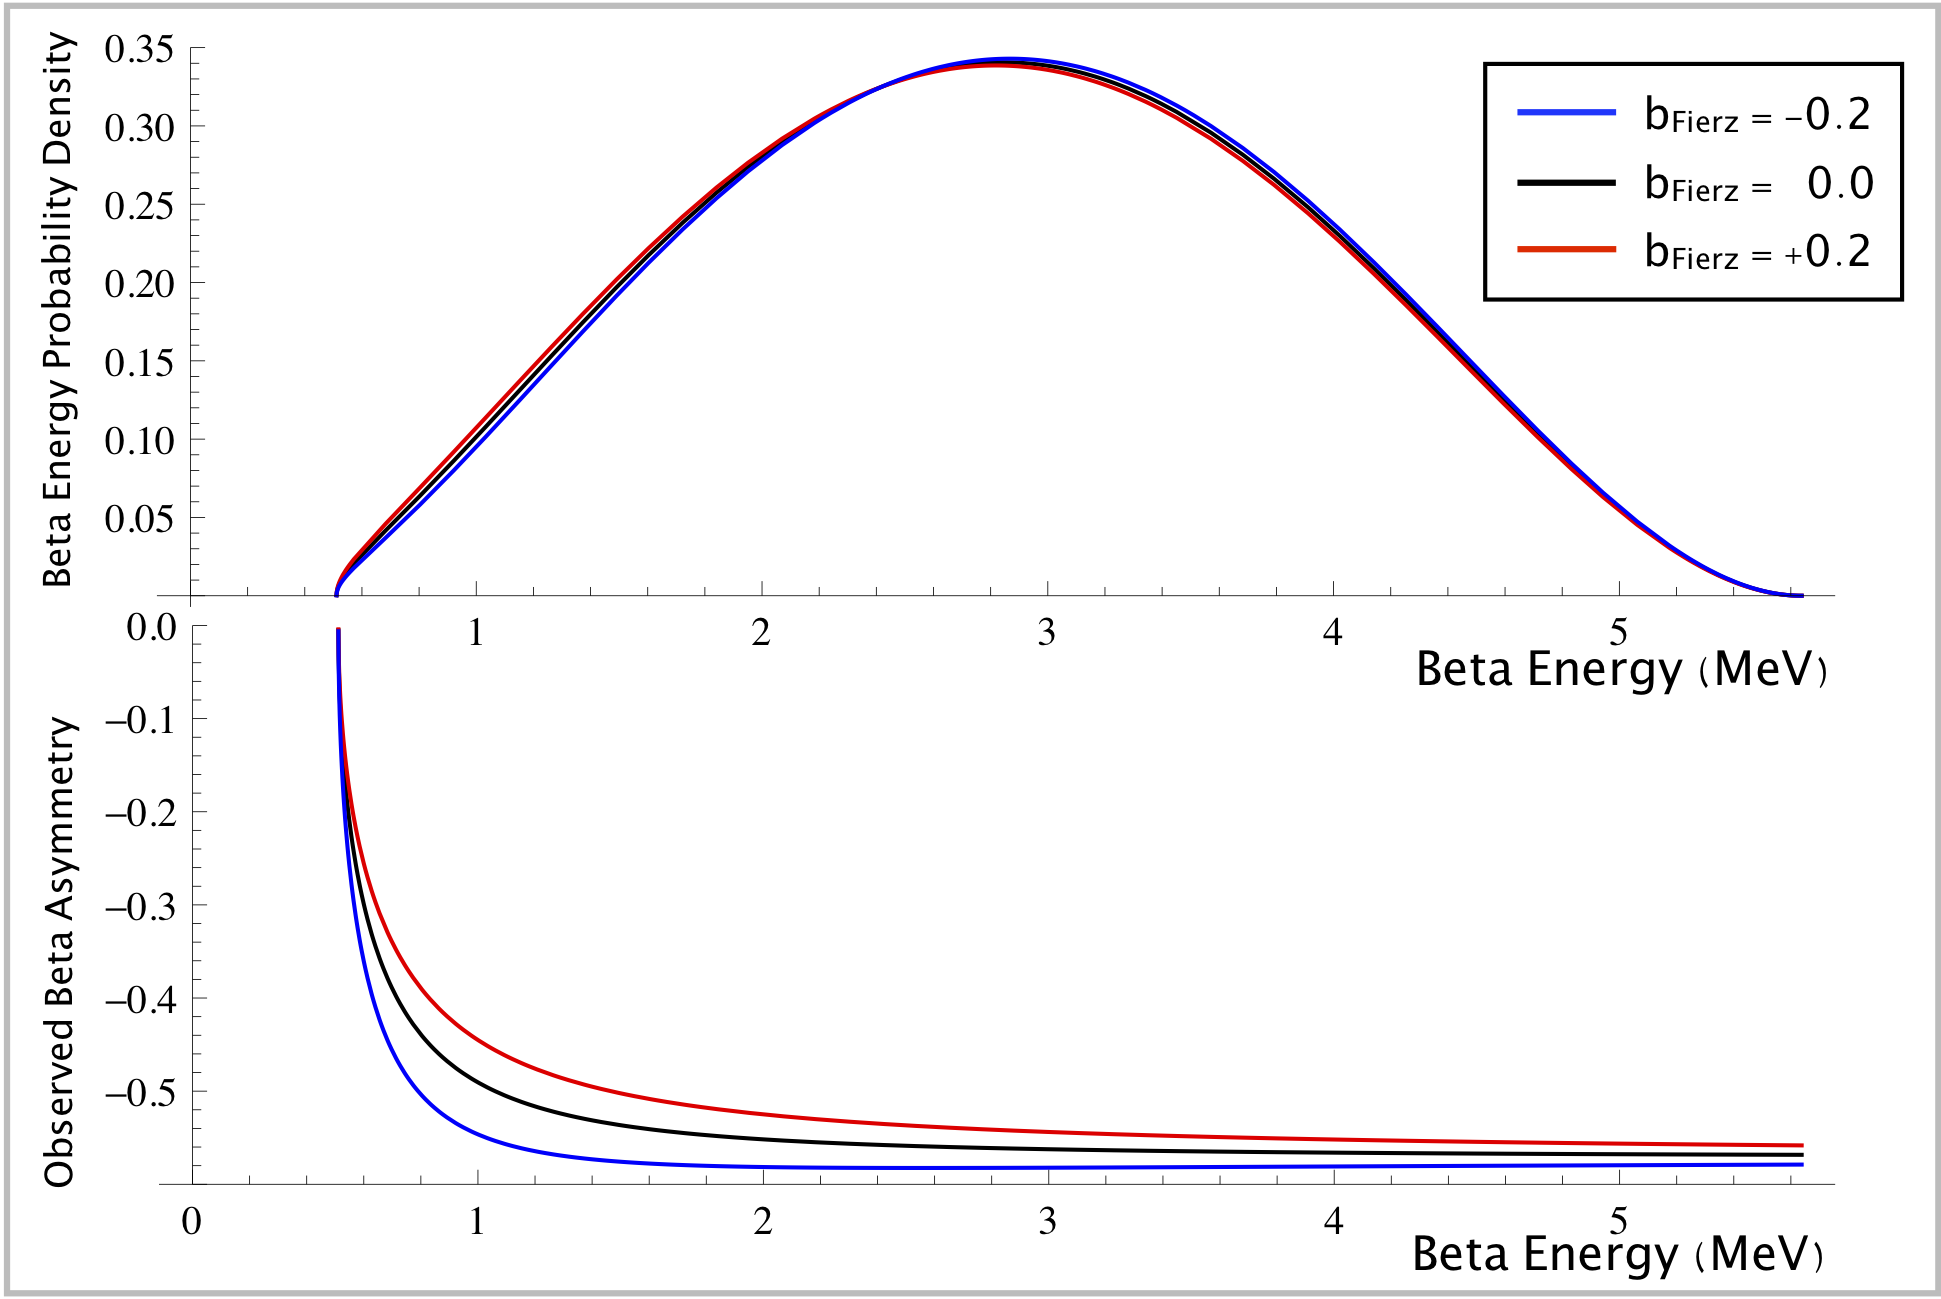
\includegraphics[width=.999\linewidth]
	{Figures/Fierz_Signature.png}
	\caption[Generated Beta Energy Spectrum and Superratio Asymmetry to Measure $\bFierz$]{A generated beta energy spectrum (top), and the superratio asymmetry associated with it (bottom) are constructed to measure a $\bFierz$ signal at the values shown.  The supersum method of Ref.~\cite{UCNA_first_Fierz} is roughly equivalent to constructing the top plot's beta energy spectrum.  Note that the magnitude of these $\bFierz$ values has been made to be unphysically large so that the effect to the top plot can be seen; both scalar and tensor couplings of the size needed to produce this effect have already been ruled out. }	\label{fig:FierzSignature}
\end{figure}


There are some limitations to what the superratio technique is able to deal with effectively, however --- notably, scattering effects don't cancel out particularly well.  Within the present project, this is a major systematic.  

Scattering, unpolarized background, \emph{and} the variety of effects effectively addressed by the superratio asymmetry construction are all included within the simulations to which the experimental data is compared, and the effects are propagated through the analysis to the end;  although many systematic effects can be reduced by the technique described above, they must still be evaluated.



\note[note,nolist]{}




%In these extremal cases, the $\bFierz$ term will account for a different \emph{fraction} of 
%\note[note,nolist]{}
%This feature of beta emission spectra hints at a potential handle we might use to measure $\bFierz$ --- as we vary the emission angle under consideration, the \emph{fractional} size of the effect we're looking for will change!

%\note[oldnote,nolist]{}
%In the TRINAT geometry with two polarization states (+/-) and two nearly equivalent detectors (T/B) aligned along the axis of polarization, we are able to describe four different count rates, with different combinations of polarization states and detectors.  Thus, neglecting beta scattering effects, we have:

%It is this latter observation which motivates the construction of the superratio and superratio asymmetry as new observables comprised of a combination of multiple physical measurements at the angular extrema of beta emission.  
%\note{
%In fact, it is possible to extract a much clearer signal to measure both $\Abeta$ and $\bFierz$ by making some clever choices in how our data should be processed.  
%}
%A further benefit to using the superratio construction, as we will soon see, is the cancellation (to first order) of many systematic effects.  The ``price'' for this reduction in systematics is, unfortunately, a decrease in statistical resolving power.  
%
%In fact, it is possible to extract a much clearer signal if we are clever with our choice of measurement.  To see this, it is helpful to notice that the \emph{overall} size of the $\bFierz$ term does not vary as a function of beta emission angle -- however, the $\Abeta$ term \emph{does}.  Indeed, in some sense, $\Abeta$ can be thought of as a parameterization of the extent to which the number of beta emissions changes as a function of angle.  
%
%The fact that we have in $\bFierz$ a small (or nonexistent), unchanging (with respect to angle) effect to be compared against a ``background'' large $\Abeta$ term which \emph{does} scale with emission angle, hints at a potential handle we might use to measure $\bFierz$ --- as we vary the emission angle under consideration, the \emph{fractional} size of the effect we're looking for will change!



\note[note,nolist]{}
%We now attempt to develop a physical intuition for the behaviour described above.  Considering Eq.~\ref{equation:integrated_jtw_INTRODUCTION}, we see that there is a beta energy dependence multiplying the $\bFierz$ term within the complete energy spectrum.  
%From this, it seems natural to assert that the most \emph{obvious} physically observable change that arises from the presence of a scalar or tensor coupling should be a change to the overall shape of the beta energy spectrum.  



%One way to do this is to separate the data into categories relating to their angular dependence with respect to the direction of nuclear spin (which parameterizes the $\Abeta$ observable).  If, as in our case, these sets of data can be further subdivided into categories that can be expected to have similar physical behaviours, but which may have differing systematic effects, the result is even more powerful.  In our case, the nuclear polarization is flipped periodically within a (mostly) symmetric apparatus, with beta detectors above and below along the axis of polarization.  The four beta spectra that result from this categorization can be used to construct a so-called superratio asymmetry.   


%The mathematical details of the superratio construction and its results are discussed in detail within Section~\ref{appendix:superratio}, so within the present section we will limit ourselves to a discussion of the results.

\note[done,nolist]{Here's where Juliette thinks I need to discuss the superratio harder.  ``On page 20, the details of the superratio construction are also relegated to an appendix''}

%%%%With the four rate spectra, $r_{D P}(\Ebeta)$, describing the rate at which events are detected in beta detector $D$ ($D =\{ \mathrm{T, B}  \}$ are the top and bottom detectors) from a decay whose parent had polarization $P$ (with $P=\{+,-\}$), we can construct the superratio asymmetry observable, $A_{\mathrm{super}}$, such that
%%%%\bea
%%%%A_{\mathrm{super}} \;\;=\;\; A_{\mathrm{super}}(\Ebeta) 
%%%%&=& \frac{ \sqrt{r_{\mathrm T-}\, r_{\mathrm B+} \phantom{ (\!\!\!\!\!) } }\; -\, \sqrt{ r_{\mathrm T+}\, r_{\mathrm B-}\phantom{ (\!\!\!\!\!) }} }{ \sqrt{r_{\mathrm T-}\, r_{\mathrm B+}\phantom{ (\!\!\!\!\!) }} \;+\, \sqrt{r_{\mathrm T+}\, r_{\mathrm B-} \phantom{ (\!\!\!\!\!) }} },
%%%%\eea
%%%%and we find the following dependence for the parameters $\Abeta$ and $\bFierz$ from Eq.~(\ref{equation:integrated_jtw_INTRODUCTION}):
%%%%\bea
%%%%A_{\mathrm{super}} &\approx& \Abeta \, \frac{v}{c} \, |\vec{P}| \, \langle | \cos\theta | \rangle \left( 1 - \bFierz \frac{mc^2}{\Ebeta} \right), 
%%%%\eea
%%%%where $v$ is the speed of the emitted beta particle, $c$ is the speed of light, $m$ is the mass of the electron, $\Ebeta$ is the total beta energy, $\vec{P}$ gives the nuclear spin-polarization vector of the parent, and $\theta$ describes the angle between the polarization vector and the direction into which the beta is emitted.  The ensemble averaged term, $\langle | \cos\theta | \rangle$, is averaged over the betas that are observed in a \emph{detector} (located along the axis of polarization).
%%%%%\note{define:  $v,c,\vec{P}, m_e,$...}


%The superratio and superratio asymmetry are discussed in detail within Section~\ref{appendix:superratio}.  The discussion includes details on which sort of systematic errors will cancel out entirely, or to leading order, with this treatment -- however 

%%It must be noted that for the present project, higher-order corrections are included in all simulations, and the effects are propagated through to the end of the analysis.  Though many systematic effects can be reduced by using the superratio asymmetry, they must still be evaluated.  Therefore, measured values of $\Abeta$ and $\bFierz$ may be directly compared to theoretical predictions.



\note{}
%%%% --- * --- %%%%

\note[done, nolist]{By normalizing Eq.~\ref{equation:integrated_jtw_INTRODUCTION} to have a conventional angular distribution 1 + (term)*$\Abeta$, we can write 
$W(\theta) = 1 + \Abeta/(1+\bFierz \E/\me) cos(\theta) 
\approx 
1 + \Abeta cos(\theta) - \bFierz \E/\me \Abeta cos(\theta) $
for small $\bFierz$.
Our  superratio observable measures directly the coefficient of the $cos(\theta)$ term., and its distortion with energy is multiplied by $\bFierz \Abeta$.
}
\note[jbn]{
The 37K $\Abeta$ is much larger than the neutron's $\Abeta$, so we gain in sensitivity compared to the neutron.
}

\note[jb1]{JB on simple things still missing:
\\
Intro or theory section:
\\...\\
P(cos(theta)) = 1 + bm/E + P  Abeta v/c cos(theta)
\\
where theta is the angle between beta and polarization direction
\\...\\
Higher-order corrections to this equation (citing your appendices and/or
chapters) are included in the simulation,
so you are extracting b and Abeta in this
equation to be compared with theory
\\...\\
\{This is a simple but vital statement-- some people actually extract Abeta(Ebeta$=$0) without recoil-order corrections, which is not the same parameter.\}
\\...\\
The theory prediction for Abeta (citing Fenker PRL) is X.
\\
The theory prediction for bFierz is 0 (maybe you have that already).
}

\note[jb1]{JB on that missing figure that I've now put in:    ``A dependence of Abeta on beta energy is also introduced.
\\
UCNA fits energy spectrum and Abeta[Ebeta] simultaneously now."
}

\note{The point is, the presence of either scalar or tensor interactions will produce a $\bFierz$ term in the decay PDF.  It has other effects on the PDF, but those come in at higher-order in the tiny scalar and tensor couplings.  So, the Fierz term would be by far the biggest thing that changes in the PDF.  The PDF describes the energy and momentum of the outgoing beta w.r.t. a variety of other things.  Notably, we can write an elegant-ish description of beta momentum w.r.t. nuclear polarization direction, and ignore the neutrino completely after integrating over it.  We have a PDF in beta \emph{direction} (w.r.t. polarization), and beta \emph{energy}.  To lowest order (and lowest order is best order) the distribution w.r.t. polarization direction doesn't change, but the distribution w.r.t. energy does change.  Or ... something?  The point is, it makes a change in the beta energy spectrum.  This change is most pronounced at low energies, because the Fierz term is scaled by $(1/\Ebeta)$.  However, the asymmetry is also a function of $\Ebeta$.  A different function of $\Ebeta$.  In fact, it is scaled by $(\pbeta/\Ebeta)$ within the PDF, which is distinctly different than $\bFierz$.  So, one might ask what effect a $\bFierz$ term would produce on a constructed asymmetry spectrum.  ....This explanation has gone way off track.}

\note[done,nolist]{JB:  You need to at some point say that the supersum is the beta energy spectrum.  There are experiments trying to do this method better, but they are very difficult.  UCNA published a combined energy spectrum and Abeta[Ebeta] analysis on the neutron in March 2020~\cite{UCNAfierz2020}.
\\...\\
MJA:  I can't help but also notice the follow-up article from September 2020~\cite{Saul2020}.  Ugh. 
}
















%%%% --- * --- %%%%	
%%%% --- * --- %%%%	
%% !TEX root = ../thesis_main.tex
%
%
%
%
%%%% --- * --- %%%%	
\chapter[SuperRatio]{Derivation of the $\bFierz$ Dependence of the Superratio Asymmetry}
\label{appendix:superratio}
\note[color=jb]{ Appendix KLM you have to pick what you want-- I hope that's Appendix K (that's this one!) -- and remove the rest as you say they're "old". Appendix K could be moved to the end of Experimental Methods because it's absolutely critical and helpful!! but if you want to reference it there and leave it as an Appendix, it's up to you.}


%Consider the following probability distribution for beta decay, which is equivalent to Eq.~(\ref{equation:integrated_jtw}).  %\aside{It's not just equivalent, it's literally identical.  }
Recall the integrated JTW probability distribution for outgoing beta particles from Eq.~(\ref{equation:integrated_jtw}):
\bea
	\textrm{d}^3 \Gamma ( \Ebeta, \mathbf{ \hat{\Omega}}_\beta ) \, \dEe \, \dOmegae
	&=& 
	\frac{2}{(2\pi)^4} \, \FF \, \pe \Ee (E_0 - \Ee)^2 \, \dEe \, \dOmegae \, \xi \nonumber\\ 
	&& \times \left[
		1 + \bFierz \frac{\m c^2}{\Ee} + 
		\A  
		\left(
			\frac{\vecJ}{J} \cdot \frac{\vecpe}{\Ee} 
		\right) 
	\right].
	\label{equation:integrated_jtw_in_superratiosection}
\eea
We note that the only angular dependence remaining in this equation is the dot product between the direction of beta emission and the direction of nuclear spin-polarization.  This allows us to pull out a further factor of $2\pi$ by choosing the axis of polarization as defining our coordinate system, and integrating over the ``$\phi_\beta$'' coordinate.  The result is a bit more friendly to work with:
%Integrating this distribution again over $\phi_\beta$, while reducing the
\bea
	\textrm{d}^2 \Gamma  ( \Ebeta, \theta ) \, \dEe \, \textrm{d} \theta %\, \dEe \, \dOmegae
	&=&
%	\frac{2}{(2\pi)^3} \, \FF \, \pe \Ee (E_0 - \Ee)^2 \, \dEe \, \dOmegae \, \xi \nonumber\\ 
%	&& \times \left[
%		1 + \bFierz \frac{\m c^2}{\Ee} + 
%		\A  
%		\left(
%			\frac{\vecJ}{J} \cdot \frac{\vecpe}{\Ee} 
%		\right) 
%	\right]
%	\\
%	&=&
	W(\Ebeta) \left[ 1 + \bFierz \frac{\m c^2}{\Ebeta} + \Abeta \, \frac{v_\beta }{c} |\vec{P}| \cos\theta  \right] \, \dEe \, \textrm{d} \theta , 
%\label{equation:integrated_jtw}
\eea
where $\theta$ is the angle between the beta emission direction and the polarization direction, and is the only angular dependence that remains.  Here, we have grouped the overall energy dependence into $W(\Ebeta)$, so that
\beq
W(\Ebeta) = \frac{2}{(2\pi)^3} \, \FF \, \pe \Ee (E_0 - \Ee)^2.
\eeq
\note{We could also use this with the Holstein formulation, at least some of it.  The point is, we can put *anything* that only depends on beta energy into $W(\Ebeta)$.  It doesn't matter, because it's already only integrable through numerical methods anyway -- so we can't possibly make it worse.}

In the TRINAT geometry with two polarization states (+/-) and two detectors (T/B) aligned along the axis of polarization, we are able to describe four different count rates, with different combinations of polarization states and detectors.  Thus, neglecting beta scattering effects, we have:
\bea
r_{\mathrm T+}(\Ebeta) &=& \varepsilon_{\mathrm T}(\Ebeta)\, \Omega_{\mathrm T} \, N_+ \left[1 + \bFierz \frac{\m c^2}{\Ebeta}  + \Abeta \, \frac{v}{c} |\vec{P}_+| \langle \cos\theta \rangle_{\mathrm T+} \right] \label{eq:r1} \\
r_{\mathrm B+}(\Ebeta) &=& \varepsilon_{\mathrm B}(\Ebeta)\, \Omega_{\mathrm B} \, N_+ \left[1 + \bFierz \frac{\m c^2}{\Ebeta}  + \Abeta \, \frac{v}{c} |\vec{P}_+| \langle \cos\theta \rangle_{\mathrm B+} \right] \label{eq:r2}\\
r_{\mathrm T-}(\Ebeta) &=& \varepsilon_{\mathrm T}(\Ebeta)\, \Omega_{\mathrm T} \, N_- \left[1 + \bFierz \frac{\m c^2}{\Ebeta}  + \Abeta \, \frac{v}{c} |\vec{P}_-| \langle \cos\theta \rangle_{\mathrm T-} \right] \label{eq:r3}\\
r_{\mathrm B-}(\Ebeta) &=& \varepsilon_{\mathrm B}(\Ebeta)\, \Omega_{\mathrm B} \, N_- \left[1 + \bFierz \frac{\m c^2}{\Ebeta}  + \Abeta \, \frac{v}{c} |\vec{P}_-| \langle \cos\theta \rangle_{\mathrm B-} \right],\label{eq:r4}
\eea
where $\varepsilon_{\mathrm T / \mathrm B}(\Ebeta)$ are the (top/bottom) detector efficiencies, $\Omega_{\mathrm T / \mathrm B}$ are the fractional solid angles for the (top/bottom) detector from the trap position, $N_{+/-}$ are the number of atoms trapped in each (+/-) polarization state, and $|\vec{P}_{+/-}|$ are the magnitudes of the polarization along the detector axis for each polarization state.  $\langle \cos\theta \rangle_{\mathrm T/ \mathrm B, +/-} $ is the average of $\cos\theta$ for \emph{observed} outgoing betas, for each detector and polarization state combination.  This latter term is approximately $\pm 1$ as a result of our detector geometry, but contains important sign information.  For a pointlike trap in the center of the chamber, 103.484 mm from either (DSSSD) detector, each of which is taken to be circular with a radius of 15.5 mm, we find that $\langle | \cos\theta | \rangle_{\mathrm T/ \mathrm B, +/-} \approx 0.994484$, and is the same for all four cases.
\aside{Not quite true.  Some strips are missing.}
% (or for $r=15.0$\,mm, we find that $\langle | \cos\theta | \rangle_{\mathrm T/ \mathrm B, +/-} \approx 0.994829$). 
\aside{This is only true if we neglect (back-)scatter.  This is not actually a good approximation.  But we have pretty good simulations to give us the real numbers, anyway. } Note that a horizontally displaced trap will decrease the magnitude of $\langle | \cos\theta | \rangle $, but as it is an expectation value of an absolute value, all four will remain equal to one another.  In the case of a vertically displaced trap, these four values will no longer all be equal, however it will still be the case that $\langle | \cos\theta | \rangle_{\mathrm T +} = \langle | \cos\theta | \rangle_{\mathrm T -}$, and $\langle | \cos\theta | \rangle_{\mathrm B+} = \langle | \cos\theta | \rangle_{\mathrm B -}$.  \aside{Is that definitely true, or is it only true to lowest order?}

In the case of the present experiment, we note that $|\vec{P}_+| = |\vec{P}_-|$ is correct to a high degree of precision.

%%%% --- * --- %%%%	

%\subsection{Derivation of the $\bFierz$ Dependence of the Superratio Asymmetry}
%\chapter[SuperRatio]{Derivation of the $\bFierz$ Dependence of the Superratio Asymmetry}
\label{appendix:superratio}
%\note[jm]{JM suggests:  Move this thing out of an appendix and into the main?}
%\note[jm]{JB on JM:  
%\\
%3. superratio:
%\\
%this is up to you. She has a point that the superratio is critical.
%You know that, and understand full details, and that's a real intellectual contribution you've made to your research.
%\\ ...\\
%You could just say it's a critical technique, say a little more qualitatively
%why it's critical (I have not re-read this) but the full lengthy details are reproducing refs. X and are best left to an appendix.
%\\
%Or as you suggest, bring it back in, because it's critical.}
%
%Recalling the beta decay \ac{PDF}'s overall energy dependence in Eq.~(\ref{eq:overallenergydependence_intro}), we note that the Fermi function $\FFminus$ at any reasonable level of approximation is integrable only by numerical methods.  As a result, there is little that could be changed to make $W(\Ebeta)$ more difficult to work with, so we can safely take $W(\Ebeta)$ to be an arbitrary function.  Therefore, for the remainder of this section, we will take $W(\Ebeta)$ to implicitly include the small corrections to overall energy dependence that arise from e.g.\! recoil-order corrections, as described by Holstein~\cite{holstein}.



\note{}
%%%we note that the only angular dependence remaining in this spectrum is the dot product between the direction of beta emission and the direction of nuclear spin-polarization.  It is therefore possible to pull out a further factor of $2\pi$ by choosing the axis of polarization as defining our coordinate system, and integrating over the $\phi_\beta$ coordinate, and Eq.~(\ref{equation:integrated_jtw_INTRODUCTION}) becomes:
%%%\bea
%%%	\textrm{d}^2 \Gamma  ( \Ebeta, \theta ) 
%%%	&=&
%%%	W(\Ebeta) \left[ 1 + \bFierz \frac{\m c^2}{\Ebeta} + \Abeta \, \frac{v_\beta }{c} |\vec{P}| \cos\theta  \right] \, \dEe \, \textrm{d} \theta , 
%%%%\label{equation:integrated_jtw}
%%%\eea
%%%where $\theta$ is the angle between the beta emission direction and the polarization direction, and is the only angular dependence that remains.  Here, we have grouped the expression's overall energy dependence into the term $W(\Ebeta)$, so that
%%%\beq
%%%W(\Ebeta) = \frac{2}{(2\pi)^3} \, \FF \, \xi \, \pe \Ee (E_0 - \Ee)^2,
%%%\label{eq:overallenergydependence}
%%%\eeq
%%%\note[tag]{this section got put verbatim into the appendix.  And also tweaked for that one previous section.  Have to put something else here.  Probably just reference it.}
%%%%where we note that the Fermi functions in the above make Eq.~\ref{eq:overallenergydependence} integrable only by numerical methods.  Because it would be difficult to make this expression \emph{more} challenging to work with, there is little drawback to including in this expression any small corrections to overall energy dependence that might arise from e.g.\! recoil-order corrections, as described by Holstein~\cite{holstein}.
%\note{We could also use this with the Holstein formulation, at least some of it.  The point is, we can put *anything* that only depends on beta energy into $W(\Ebeta)$.  It doesn't matter, because it's already only integrable through numerical methods anyway -- so we can't possibly make it worse.}

%%%%In the TRINAT geometry with two polarization states (+/-) and two nearly equivalent detectors (T/B) aligned along the axis of polarization, we are able to describe four different count rates, with different combinations of polarization states and detectors.  Thus, neglecting beta scattering effects, we have:
%%%%\bea
%%%%r_{\mathrm T+}(\Ebeta) &=& W(\Ebeta) \varepsilon_{\mathrm T}(\Ebeta)\, \Omega_{\mathrm T} \, N_+ \left[1 + \bFierz \frac{\m c^2}{\Ebeta}  + \Abeta \, \frac{v}{c} |\vec{P}_+| \langle \cos\theta \rangle_{\mathrm T+} \right] \label{eq:r1} \\
%%%%r_{\mathrm B+}(\Ebeta) &=& W(\Ebeta) \varepsilon_{\mathrm B}(\Ebeta)\, \Omega_{\mathrm B} \, N_+ \left[1 + \bFierz \frac{\m c^2}{\Ebeta}  + \Abeta \, \frac{v}{c} |\vec{P}_+| \langle \cos\theta \rangle_{\mathrm B+} \right] \label{eq:r2}\\
%%%%r_{\mathrm T-}(\Ebeta) &=& W(\Ebeta) \varepsilon_{\mathrm T}(\Ebeta)\, \Omega_{\mathrm T} \, N_- \left[1 + \bFierz \frac{\m c^2}{\Ebeta}  + \Abeta \, \frac{v}{c} |\vec{P}_-| \langle \cos\theta \rangle_{\mathrm T-} \right] \label{eq:r3}\\
%%%%r_{\mathrm B-}(\Ebeta) &=& W(\Ebeta) \varepsilon_{\mathrm B}(\Ebeta)\, \Omega_{\mathrm B} \, N_- \left[1 + \bFierz \frac{\m c^2}{\Ebeta}  + \Abeta \, \frac{v}{c} |\vec{P}_-| \langle \cos\theta \rangle_{\mathrm B-} \right],\label{eq:r4}
%%%%\eea
%%%%where $\varepsilon_{\mathrm T / \mathrm B}(\Ebeta)$ are the (top/bottom) detector efficiencies, $\Omega_{\mathrm T / \mathrm B}$ are the fractional solid angles for the (top/bottom) detector from the trap position, $N_{+/-}$ are the number of atoms trapped in each (+/-) polarization state, and $|\vec{P}_{+/-}|$ are the magnitudes of the polarization along the detector axis for each polarization state.  $\langle \cos\theta \rangle_{\mathrm T/ \mathrm B, +/-} $ is the average of $\cos\theta$ for \emph{observed} outgoing betas, for each detector and polarization state combination.  This latter term is approximately $\pm 1$ as a result of our detector geometry, but contains important sign information.  




%We define the superratio, $s$, to be:
%\bea
%s \;\;=\;\; s(\Ebeta) \;\;:=\;\; \frac{ r_{\mathrm T+}\, r_{\mathrm B-} }{ r_{\mathrm T-}\, r_{\mathrm B+} }, 
%\eea
%and the superratio asymmetry, $A_{\mathrm{super}}$, as
%\bea
%A_{\mathrm{super}} \;\;=\;\; A_{\mathrm{super}}(\Ebeta) &:=& \frac{1-\sqrt{s}}{1+\sqrt{s}} 
%\\
%&=& \frac{ \sqrt{r_{\mathrm T-}\, r_{\mathrm B+} \phantom{ (\!\!\!\!\!) } }\; -\, \sqrt{ r_{\mathrm T+}\, r_{\mathrm B-}\phantom{ (\!\!\!\!\!) }} }{ \sqrt{r_{\mathrm T-}\, r_{\mathrm B+}\phantom{ (\!\!\!\!\!) }} \;+\, \sqrt{r_{\mathrm T+}\, r_{\mathrm B-} \phantom{ (\!\!\!\!\!) }} }
%\eea
%%
%This is explicitly an experimental quantity that is measured directly by the above combination of count rates, however it is obvious that it reduces, under appropriate limits, to be equivalent to a naive asymmetry.  In particular, if we require that the physical conditions and relative detector positions and sensitivities are identical when the polarization is flipped, then we have $r_{\mathrm T+}(\Ebeta) = r_{\mathrm B-}(\Ebeta)$ and $r_{\mathrm T-}(\Ebeta) = r_{\mathrm B+}(\Ebeta)$.
%%
%It follows that we can simplify the superratio asymmetry into a more intuitive quantity that we might use for a measurement with only a single polarization state, e.g.,  
%\bea
%A_{\mathrm{super}, +} &\rightarrow& \frac{ r_{\mathrm T}\, - \,r_{\mathrm B} }{r_{\mathrm T}\, +\, r_{\mathrm B} }. 
%\label{eq:singlepol_asymmetry}
%\eea

%\note[note, nolist]{begin thing I haven't yoinked from yet:  }
%%%While Eq.~\ref{eq:singlepol_asymmetry} is conceptually encouraging, the assumptions that gave rise to that expression are too simplifying.  We will introduce some more limited assumptions for what follows, along with shorthand notation for improved readability.  First, we require that the magnitude of the polarization vector is the same for both polarization states, and also that the average of the magnitude of $\cos\theta$ for a given detector does not change when the polarization is flipped (equivalent to a requirement that the trap position doesn't change when the polarization is flipped).  Then: 
%%%\bea
%%%P &:=& |\vec{P}_+| = |\vec{P}_-|  \\
%%%\langle |\cos\theta | \rangle_T &:=& \langle |\cos\theta | \rangle_{\mathrm T+} \, = \, \langle |\cos\theta | \rangle_{\mathrm T-} \\
%%%\langle |\cos\theta | \rangle_B &:=& \langle |\cos\theta | \rangle_{\mathrm B+} \, = \, \langle |\cos\theta | \rangle_{\mathrm B-},
%%%\eea
%%%and we can further define
%%%\bea
%%%c &=& \,\,\,\,\, \langle | \cos\theta | \rangle :=  \frac{1}{2} \left( \phantom{2_2^2}\!\!\!\! \langle |\cos\theta | \rangle_T + \langle |\cos\theta | \rangle_B \, \right) \\
%%%\Delta c &=& \Delta \langle | \cos\theta | \rangle := \frac{1}{2} \left( \phantom{2_2^2}\!\!\!\! \langle |\cos\theta | \rangle_T - \langle |\cos\theta | \rangle_B \, \right)
%%%\eea
%%%and 
%%%\bea
%%%\tilde{A} &=\;\; \tilde{A}(\Ebeta) &:=\;\; A_\beta \frac{v}{c} \\ 
%%%\tilde{b} &=\;\; \tilde{b}(\Ebeta) &:=\;\;  \bFierz \frac{mc^2}{\Ebeta}, \\
%%%\tilde{r} &=\;\; \tilde{r}(\Ebeta) &:=\;\; 1+\tilde{b}. 
%%%\eea
%%%
%%%With this new set of variables defined, we can re-write Eqs.~(\ref{eq:r1}-\ref{eq:r4}) as
%%%\bea
%%%r_{\mathrm T+}(\Ebeta) &=& W(\Ebeta)\, \varepsilon_{\mathrm T}(\Ebeta)\, \Omega_{\mathrm T}\, N_+ \left[\tilde{r}  \,+\, \tilde{A} P \left( \phantom{2_2^2}\!\!\!\! c + \Delta c \, \right) \right] \\
%%%r_{\mathrm B+}(\Ebeta) &=& W(\Ebeta)\, \varepsilon_{\mathrm B}(\Ebeta)\, \Omega_{\mathrm B}\, N_+ \left[\tilde{r}  \,-\, \tilde{A} P \left( \phantom{2_2^2}\!\!\!\! c - \Delta c \, \right) \right] \\
%%%r_{\mathrm T-}(\Ebeta) &=& W(\Ebeta)\, \varepsilon_{\mathrm T}(\Ebeta)\, \Omega_{\mathrm T}\, N_- \left[\tilde{r}  \,-\, \tilde{A} P \left( \phantom{2_2^2}\!\!\!\! c + \Delta c \, \right) \right] \\
%%%r_{\mathrm B-}(\Ebeta) &=& W(\Ebeta)\, \varepsilon_{\mathrm B}(\Ebeta)\, \Omega_{\mathrm B}\, N_- \left[\tilde{r}  \,+\, \tilde{A} P \left( \phantom{2_2^2}\!\!\!\! c - \Delta c \, \right) \right], 
%%%\eea
%%%and the superratio becomes
%%%\bea
%%%s 
%%%&=& 
%%%\frac{ 
%%%\left(
%%%\tilde{r} + \tilde{A} P c \right)^2 -  \left( \phantom{\tilde{2}_2^2}\!\!\!\!\! \Delta c \right)^2 
%%%}{ 
%%%\left(
%%%\tilde{r} - \tilde{A} P c \right)^2 -  \left( \phantom{\tilde{2}_2^2}\!\!\!\!\! \Delta c \right)^2 
%%%} 
%%%\eea
%%%where all factors of $W(\Ebeta)$, $\varepsilon_{\mathrm T/B}(\Ebeta)$, $\Omega_{\mathrm T/B}$, and $N_{+/-}$ have been cancelled out entirely.  

%For simplicity we take $\Delta c = 0$ in what follows.  Although this is not strictly accurate within the present experiment, this assumption greatly simplifies the expressions that follow.  Then, absent other corrections (\emph{e.g.} backscattering, unpolarized background, ...), it is clear that if $\tilde{b} = 0$ as in the Standard Model, %it follows that 
%\bea
%A_{\mathrm{super}} &=\;\; \tilde{A} P c &=\;\; \Abeta \, \frac{v}{c} \, |\vec{P}| \, \langle | \cos\theta | \rangle
%\eea
%
%In the case where $\tilde{b} \neq 0$, we find that 
%\bea
%A_{\mathrm{super}} &=& \frac{\tilde{A} P c}{1+\tilde{b}} \\
%&\approx&  \tilde{A} P c \, (1 - \tilde{b} + {\tilde{b}}^2),
%\eea
%where we have utilized the assumption that $\tilde{b} \ll 1$.
%Thus, to leading order in terms of $\tilde{b}$, 
%\bea
%A_{\mathrm{super}} &\approx& \Abeta \, \frac{v}{c} \, |\vec{P}| \, \langle | \cos\theta | \rangle \left( 1 - \bFierz \frac{mc^2}{\Ebeta} \right).
%\eea














%%%% %%%% %%%% %%%% %%%% %%%%
%%%% %%%% %%%% %%%% %%%% %%%%
\ifthenelse{\boolean{isdraft}}
{
	\pagebreak
}
{}
%%%% %%%% %%%% %%%% %%%% %%%%
\section{The Gamow-Teller/Fermi Mixing Ratio and Related Constraints}
\label{sec:extractinglambda}
It is clear from Sec.~\ref{sec:mathdescription_intro} that in order to make a prediction about the behaviour of outgoing particles within a particular beta decay transition, it is fundamentally important to know the value of the mixing ratio $\rho$.

Of course, it is possible to perform a relatively direct measurement of $\rho$ through an observation of one of the other \ac{JTW} parameters (e.g., a measurement of $\Abeta$ in combination with Eq.~(\ref{eq:Awithrho_intro}) rapidly leads to a value for $\rho$.).  However, this strategy has certain drawbacks -- notably, the apparatus required to perform such a measurement \emph{well} must be fairly complex;  the TRINAT setup, for example, cannot readily be used with isotopes of most chemical elements.  

For $^{37}$K in particular, this direct approach \emph{has} been used in the past, both with the present dataset as well as with previously collected data, yielding an overall value of $\rho=0.576 \pm 0.006$~\cite{ben_Abeta}\cite{shidling2014}\cite{dan_Bnu}.

As we do not wish to re-use the same data twice within a single measurement, we take as our baseline the value of $\rho$ as extracted in a more roundabout way as described below.


It is useful to define the strength, $ft$, of a transition --- also known as the $ft$ value.  This is fundamentally an experimental quantity.  Though the $ft$ value is in principle the product of two quantities --- the statistical rate function $f$ and the partial half-life $t$ --- it is common to treat the product as a single unit.  
%The $ft$ value then can be directly related to the fundamental vector coupling strength.  
%
The statistical rate function $f$ must be split into vector and axial components ($f_V$ and $f_A$) in order be evaluated, and $f_V$ in particular is often used alone, as we will see below.  The statistical rate functions are, in essence, integrals over the accessible lepton phase space, and both $f_V$ and $f_A$ are mathematically non-trivial objects\cite{towner_hardy_1995_frombook}\cite{HardyTowner2005_Superallowed}, but can be evaluated by, e.g., the methods of Refs.~\cite{wilkinson2}\cite{wilkinson3}\cite{wilkinson4}.  
%Both vector and axial statistical rate functions are mathematically non-trivial objects\cite{towner_hardy_1995_frombook}\cite{HardyTowner2005_Superallowed}, but can be evaluated by, e.g., the methods of Refs.~\cite{wilkinson2}\cite{wilkinson3}\cite{wilkinson4}.  
Such calculations are beyond the scope of the present work, however we will note that 
%For our purposes here, we will simply note that 
$f_V$ and $f_A$ are characterized primarily by the beta endpoint energy $E_0$ (scaling as $\sim E_0^5$), a quantity which can readily be measured.\aside[note]{John said this.  But I should probably cite someone here.}  

The partial half-life $t$ can be quickly calculated given knowledge of the total half-life $t_{1/2}$ and branching ratio $R$, as:
\bea
t &=&  \frac{1}{R} \, (1 + P_{\mathrm{EC}}) \,\, t_{1/2}, 
\eea
where $P_{\mathrm{EC}}$ is the electron capture probability (in the case of $^{37}$K, $P_{\mathrm{EC}}=0.0008$ makes only a small contribution~\cite{SeverijnsTandecki2008}).  
\aside{could also cite Severijns2008's Refs. 35 and 36...}  
It is also possible to write down an expression for $t$ based on something closer to a first principles approach:  
%,  including corrections arising from a variety of physical effects:
\bea
t &=& \frac{K}{ G_F^2 \, V_{ud}^2  \left( f_V\, C_V^2 |M_F|^2 + f_A\, C_A^2 |M_{GT}|^2 
%\phantom{\frac{1^1_1}{1^1_1} \!\!\!\!\!\! } 
\right) }.
\label{eq:partialhalflife_theory}
\eea
Here, $K = (\hbar c)^6 2\pi^3 \hbar \ln(2) (\me c^2)^{-5}$ is a simple combination of physical constants, and, as described in Sec.~\ref{sec:mathdescription_intro}, $C_V$ ($C_A$) is the universal complex coupling parameter associated with vector (axial) currents, while $M_F$ ($M_{GT}$) is the transition matrix element associated with vector (axial) coupling for a specific decay.
%are as described in \emph{e.g.} Section~\ref{sec:mathdescription_intro}.  
$G_F$ is the weak interaction coupling constant, which is measured experimentally through muon decay.  $V_{ud}$ is the up-down mixing element within the \ac{CKM} matrix; its precise determination is an active area of research, motivated in part by the attempt to search for or constrain the possible presence of a fourth generation of quarks.  

It is worthwhile, at this stage, to briefly discuss the corrections to the Fermi and Gamow-Teller matrix elements, $M_F$ and $M_{GT}$, that have already been implicitly applied.  Although the uncorrected matrix elements $M_F^0$ and $M_{GT}^0$ are in some sense the more fundamental quantities, the corrected matrix elements are what is measured by an experiment.  $M_F^0$ and $M_{GT}^0$ are related to their corrected counterparts according to:
\bea
|M_F|^2    &=& (1+\delta_R^\prime) (1 + \delta_{NS}^V - \delta_C^V) (1+\Delta_R^V) \, |M_F^0|^2
\label{eq:MF_expand}
\\
|M_{GT}|^2 &=& (1+\delta_R^\prime) (1 + \delta_{NS}^A - \delta_C^A) (1+\Delta_R^A) \, |M_{GT}^0|^2 , 
\label{eq:MGT_expand}
\eea 
where $\delta_C^{V}$ ($\delta_C^{A}$) is the isospin symmetry breaking correction for the vector (axial-vector) current.  Here, $\delta^\prime_R$ is the portion of the outer radiative correction (\emph{i.e.}, it is dependent on the specific transition in question) that depends \emph{only trivially} on the nucleus; it is identically the same for vector and axial couplings.  The $\delta_{NS}^V$ ($\delta_{NS}^A$) term is the portion of the outer radiative correction for the vector (axial-vector) current with a \emph{non-trivial} dependence on nuclear structure.  These require a detailed shell model calculation to evaluate, as described in \emph{e.g.}  Refs.~\cite{TownerHardy2008}\cite{JausRasche1990}\cite{barker1992}\cite{Towner1992}\cite{Towner1994}.  Finally, the quantities $\Delta_R^V$ and $\Delta_R^A$ arise from inner radiative corrections (\emph{i.e.}, independent of the specific transition being considered) to the vector and axial-vector currents, and may be calculated as in Refs.~\cite{MarcianoSirlin_1986}\cite{MarcianoSirlin_2006}\cite{CzarneckiMarcianoSirlin_2019}\cite{Hayen2021}.  Although they do not depend on the specifics of any transition, the $\Delta_R^V$ and $\Delta_R^A$ terms are included here within the expressions for (transition-specific) $M_F$ and $M_{GT}$ for our later convenience.  This convention is sometimes, but not always, followed within the published literature~\cite{SeverijnsTandecki2008}\cite{HardyTownerSuperallowed2020}. 

%%\note[note,nolist]{}
%%$\delta_C^{V}$ is the isospin symmetry breaking correction for the vector current, $\delta^\prime_R$ is the portion of the outer radiative correction (ie, dependent on the specific nucleus in question) that depends only trivially on the nucleus, 
%%and $\delta_{NS}^{V}$ is the portion of the outer radiative correction %(depends on the specific nucleus) 
%%to the vector current that depends in a \emph{non-trivial} way on nuclear structure and requires a detailed shell model calculation to evaluate, as described in e.g.  Refs.~\cite{TownerHardy2008}\cite{JausRasche1990}\cite{barker1992}\cite{Towner1992}\cite{Towner1994}.  
%%\note[note,nolist]{}


We will now consider the special case of superallowed $0^+ \rightarrow 0^+$ decay (of which $^{37}$K is \emph{not} an example).  As a general rule, these are strong, clean transitions which proceed only through vector coupling with no axial components.  Quantitatively, this amounts to setting $M_{GT}^0=0$ and $M_F^0=2$ within Eq.~(\ref{eq:partialhalflife_theory}).  As always, $C_V=1$ by construction.  With all axial couplings eliminated completely, the superallowed $0^+ \rightarrow 0^+$ decays are
%As such, they are 
%%very well suited to extract (using other experimentally measured parameters) a measure of the fundamental vector coupling strength.  
ideal candidates for measurements of the fundamental vector coupling strength.
If the \ac{CVC} hypothesis holds (and there is some reason to believe that it does~\cite{severijns_beck_cuncic_2006}\cite{HardyTownerSuperallowed2020}), then this coupling strength is common to \emph{all} transitions.  We will soon see how knowledge of this absolute vector coupling strength taken from measurements of $0^+ \rightarrow 0^+$ decay allows us to make predictions about the decay of $^{37}$K as well.  
\note[done,nolist]{My apologies for speculating more needs to be said about $0^+ \rightarrow 0^+$ -- that's not her main concern-- but it might help to add a further qualitative sentence after
\\
`then this coupling strength is common to all transitions.'
\\
with something like
\\
`We will need this absolute strength for the vector part of 37K decay when we get the ratio of vector and axial vector matrix elements from our fT value and predict our observables.'
}

In practice, the $ft$ values measured in superallowed $0^+ \rightarrow 0^+$ transitions need some small corrections in order to arrive at a universally applicable measure of the vector coupling strength.  We define a corrected $ft$ value for these transitions, $\mathcal{F}t^{0^+\!\rightarrow0^+}$ (sometimes simply $\mathcal{F}t$), as:
\bea
\mathcal{F}t^{0^+\!\rightarrow0^+} &:=& 
\left( f_V t \right) 
\!
\Bigg\rvert_{0^+\!\rightarrow0^+_{\phantom .}}
\!\!\!\!\!\! \!\!\!\!\!\! 
(1 + \delta^\prime_R)(1 + \delta_{NS}^V - \delta_C^{V} ) 
\label{eq:Ft_with_fVt}\\
&=& 
\frac{K \phantom{x^{x^x}_x} }{2 \, G_F^2 \, V_{ud}^2 (1+\Delta_R^V) } , 
\label{eq:Ft_with_Vud}
\eea
where we have made use of Eq.~(\ref{eq:partialhalflife_theory}).  
\aside[note]{I think we've probably assumed something like 
\\
$C_V |M_F^0|_{0^+\!\rightarrow0^+} = 2$ ? } 
Within Eqs.~(\ref{eq:Ft_with_fVt})-(\ref{eq:Ft_with_Vud}) above, only the parameters $t$ and $G_F$ are measured directly, while the other parameters must be calculated.  If all measurements and calculations have been performed perfectly, then Eq.~(\ref{eq:Ft_with_fVt}) is expected to yield the same $\mathcal{F}t$-value for \emph{any} superallowed $0^+ \rightarrow 0^+$ transition, as the contributions from nuclear structure have all been removed.  The above relationship is commonly used to extract an experimental value for $V_{ud}$, which cannot be calculated directly.

While Eq.~(\ref{eq:Ft_with_Vud}) describes physical parameters that are universal, it is important to remember that we have only arrived at this result by specializing our description to the superallowed $0^+ \rightarrow 0^+$ transitions; Eqs.~(\ref{eq:Ft_with_fVt})-(\ref{eq:Ft_with_Vud}) are not applicable as-is to other types of transitions.  %, so the nuclear structure parameters of Eqs.~(\ref{eq:Ft_with_fVt})-(\ref{eq:Ft_with_Vud}) must only be evaluated for this same class of decays.  
It is, however, also possible to write down an analogous expression to describe the universal vector coupling strength using parameters related to other types of decays.  As the axial current is not conserved, we will still only be interested in the vector components of such transitions, and it will take a bit more work to separate these out within a transition where both couplings contribute.  We will consider the mixed (Fermi/Gamow-Teller) mirror decays (of which $^{37}$K \emph{is} an example).  Again, $C_V=1$ (it is a universal parameter), however for the case of mirror transitions, $M_F^0 = 1$ and $M_{GT}\neq0$.

It is useful, at this stage, to recall the definition of $\rho$, the axial-vector/vector mixing ratio for a specific transition from Eq.~(\ref{eq:definerho_intro}).  In the notation of Eqs.~(\ref{eq:MF_expand})-(\ref{eq:MGT_expand}), we have:
\bea
\rho &:=& \frac{C_A \, M_{GT} }{C_V \, M_F} 
\nonumber
\\
&=& \frac{C_A \, M_{GT}^0 }{C_V \, M_F^0}  \left[ \frac{(1 + \delta_{NS}^A - \delta_C^A) }{(1 + \delta_{NS}^V - \delta_C^V)} \frac{(1+\Delta_R^A)}{(1+\Delta_R^V)} \right]^{1/2}
\label{eq:rho_with_corrections}
\\
&\approx& \frac{C_A \, M_{GT}^0 }{C_V \, M_F^0}.
\eea


As before, we use Eq.~(\ref{eq:partialhalflife_theory}) to write down $f_V t$, this time for the mixed mirror \mbox{transitions}:
\bea
( f_V t ) \Bigg\rvert_{\mathrm{mirror}_{\phantom .}}
\!\!\!\!\!\! \!\!\!\!\!\! 
&=& 
\frac{K}{G_F^2 V_{ud}^2 C_V^2 |M_F|^2 \left(1 + \frac{f_A}{f_V}\rho^2 \right)}
\\
&=& 
\frac{K}{G_F^2 V_{ud}^2 (1 + \delta^\prime_R) (1 + \delta_{NS}^V - \delta_C^V)(1+\Delta_R^V) \left(1 + \frac{f_A}{f_V}\rho^2 \right)} 
\;\;\;\; 
%\frac{K}{G_F^2 V_{ud}^2 C_V^2 |M_F|^2 \left(1 + \frac{f_A}{f_V}\frac{C_A^2}{C_V^2} \frac{|M_{GT}|^2}{|M_F|^2} \right)}.  
\eea
We now define a corrected $\mathcal{F}t$ value, $\mathcal{F}t^{\mathrm{mirror}}$, for mirror transitions by 
applying the same nuclear structure corrections that were used in Eq.~(\ref{eq:Ft_with_fVt}).  Then:
\bea
\!\!\!\! \!\!\!\!
\mathcal{F}t^{\mathrm{mirror}} &:=& 
( f_V t ) \Bigg\rvert_{\mathrm{mirror}_{\phantom .}}
\!\!\!\!\!\! \!\!\!\!\!\! 
(1 + \delta^\prime_R)(1 + \delta_{NS}^V - \delta_C^{V} ) 
\nonumber \\
&=& 
\frac{K}{G_F^2 V_{ud}^2 (1+\Delta_R^V)
\left(1 + \frac{f_A}{f_V}\rho^2 \right) } 
\label{eq:Ftmirror_withVud}
%\frac{K}{G_F^2 V_{ud}^2 C_V^2 |M_F^0|^2 (1+\Delta_R^V)
%\left(1 + \frac{f_A}{f_V}\frac{C_A^2}{C_V^2} \frac{|M_{GT}^0|^2}{ |M_F^0|^2} \frac{(1 + \delta_{NS}^A - \delta_C^A) }{(1 + \delta_{NS}^V - \delta_C^V)} \frac{(1+\Delta_R^A)}{(1+\Delta_R^V)} \right) } 
\eea

Using a measured value of $\rho$, it is possible to extract a measurement of $V_{ud}$ from Eq.~(\ref{eq:Ftmirror_withVud}) above.  However, as a separate measurement of $\rho$ is not always available, it is perhaps more common to approach the above result as a way to \emph{find} $\rho$.  Comparing with Eqs.~(\ref{eq:Ft_with_Vud}) and (\ref{eq:Ftmirror_withVud}):  
\bea
\mathcal{F}t^{0^+\!\rightarrow0^+}
&=& 
\frac{1}{2} \left(1 + \frac{f_A}{f_V}\rho^2 \right) \mathcal{F}t^{\mathrm{mirror}}.
\label{eq:Ft_and_Ftmirror}
\eea
We see, perhaps counterintuitively, that Eq.~(\ref{eq:Ft_and_Ftmirror}) makes it possible to extract the value of $\rho$ for one transition by using (in part) information measured in an entirely separate class of transitions.  

Of course, this method for evaluating $\rho$ relies on the accuracy and precision of the theoretical calculations involved to reach this point.  It is worth noting that the lepton phase space integrals $f_V$ and $f_A$ for vector and axial couplings, which directly affect the extracted value of $\rho$ in Eq.~(\ref{eq:Ft_and_Ftmirror}) above, are identically the same under the allowed approximation.  However, when higher-order corrections are taken into account, they are found to differ by $\sim 0.9\%$ for the primary $^{37}$K decay branch~\cite{HayenSeverijns2019}.



\note[note,nolist]{}
%\note[tag]{Now just *say some stuff* about the various Ft values.}
\note[note,nolist]{}

%Here, $f_A$ and $f_V$ are integrals over the lepton phase space for the axial vector and vector parts. Those integrals are identical in the allowed approximation, but differ by X\% when higher-order terms are taken into account~\cite{Hayen2021}.
%(see Appendix~\ref{appendix_forthepeople}, Refs.~\cite{holstein},~\cite{Hayen2021}.)
\note[tag]{$f_A$ and $f_V$ with higher-order terms.  X\%.  See Hayen2021.  Or, perhaps, HayenSeverijns2019?  }


%%%%\color{skyblue}The uncorrected Fermi matrix element $M_F^0$ is related to quantities that have already been defined by $| M_F |^2 =  (1 + \delta^\prime_R)(1 + \delta_{NS}^V - \delta_C^{V} ) | M_F^0 |^2 $.  
%%%%\color{black}
%With Eq.~(\ref{eq:rhorelation}), the value of $\rho$ in a mirror decay is described in terms of physical observables from an entirely separate class of decay transitions, as well as its own half-life and branching ratio.  Alternately, with a separate measurement of $\rho$, a check can be performed on the value of $V_{ud}$.
%%~\aside{this would be a good place to cite a bunch of people.}
\note[bluetodo,nolist]{}


%Comparing this with Eq.~(\ref{eq:Ft_with_Vud}), it is clear that these two expressions are closely related:
%\bea
%\mathcal{F}t^{\mathrm{mirror}}
%&=& 
%\frac{2 \mathcal{F}t^{0^+\!\rightarrow0^+} }{ \left(1 + \frac{f_A}{f_V}\rho^2 \right) }
%\eea


%%%\bea
%%%\rho &:=& \frac{C_A}{C_V} \frac{|M_{GT}|}{ |M_F|}
%%%\\
%%%&=& \frac{C_A}{C_V} \frac{|M_{GT}^0|}{ |M_F^0|} \left[ \frac{(1 + \delta_{NS}^A - \delta_C^A) }{(1 + \delta_{NS}^V - \delta_C^V)} \frac{(1+\Delta_R^A)}{(1+\Delta_R^V)} \right]^{1/2}
%%%\label{eq:rho_with_corrections}
%%%\\
%%%&\approx& \frac{C_A |M_{GT}^0| }{C_V |M_F^0|}.
%%%\eea
%
%The careful reader may notice that Eq.~(\ref{eq:rho_with_corrections}) is not \emph{quite} equivalent to the definition of $\rho$ provided in Eq.~(\ref{eq:definerho_intro}).  
%In fact, within the literature, the 
%
%\note[bluetodo]{JFC, I broke math.  .... no, I think it's actually ok.}
%\aside[note]{We haven't put this in yet, but eventually we'll probably have $C_V |M_F^0|_{\mathrm{mirror}} = 1$ ? }
%\aside[note]{*Probably* we have  $C_V = M_F^0 = 1$ by construction?  }
%

%%%%\color{skyblue}
%%%%Then Eq.~(\ref{eq:rho_with_corrections}) becomes:
%%%%\bea
%%%%\mathcal{F}t^{\mathrm{mirror}} 
%%%%&=& 
%%%%\frac{K}{G_F^2 V_{ud}^2 C_V^2 |M_F^0|^2 (1+\Delta_R^V) 
%%%%\left(1 + \frac{f_A}{f_V} \rho^2 \right) } 
%%%%\eea
%%%%
%%%%%\note[note]{And.... now what?\\ The important thing is... to be careful about what goes where?  Or something?\\ Or, maybe the inner radiative corrections were *always* there.  idk.  maybe Hayen addresses this?  But I can't quite turn his notation into something like this.}
%%%%
%%%%\bea
%%%%\mathcal{F}t &=& f_V t \, (1 + \delta^\prime_R)(1 + \delta_{NS}^V - \delta_C^{V} ),
%%%%\label{eq:define_Ft}
%%%%\eea
%%%%where 
%%%%$\delta_C^{V}$ is the isospin symmetry breaking correction for the vector current, 
%%%%$\delta^\prime_R$ is the portion of the outer radiative correction (ie, dependent on the specific nucleus in question) that depends only trivially on the nucleus, 
%%%%and
%%%%$\delta_{NS}^{V}$ is the portion of the outer radiative correction %(depends on the specific nucleus) 
%%%%to the vector current that depends in a \emph{non-trivial} way on nuclear structure and requires a detailed shell model calculation to evaluate, as described in e.g.  Refs.~\cite{TownerHardy2008}\cite{JausRasche1990}\cite{barker1992}\cite{Towner1992}\cite{Towner1994}.  
%%%%We have of course implicitly specialized the $\mathcal{F}t$ value to consider only the vector component of the statistical rate function, but this is redundant in the case of the superallowed $0^+ \rightarrow 0^+$ transitions that are presently under consideration.
%%%%
%%%%Within Eq.~\ref{eq:define_Ft}, we have corrected away all contributions from nuclear structure, and what remains can also be described in terms of fundamental couplings as:
%%%%\bea
%%%%\mathcal{F}t &=& \frac{K}{2 \, G_V^2 (1+\Delta_R^V) },
%%%%\label{eq:relate_Ft_to_couplings}
%%%%\eea
%%%%with $K$ a rather messy combination of physical constants: $K = (\hbar c)^6 2\pi^3 \hbar \ln(2) (\me c^2)^{-5}$.  
%%%%%
%%%%In Eq.~\ref{eq:relate_Ft_to_couplings} above, $G_V$ is the vector coupling constant for semileptonic weak interactions, and $\Delta_R^{V}$ is the vector current's inner radiative correction (independent of the specific transition being considered), calculated as in e.g. Refs.~\cite{MarcianoSirlin_1986}\cite{MarcianoSirlin_2006}\cite{CzarneckiMarcianoSirlin_2019}.  %$\Delta_R^{V}$
%%%%
%%%%We can also relate the vector coupling constant $G_V$ to two other experimental observables:
%%%%\bea
%%%%G_V = V_{ud}  \, G_F
%%%%\label{eq:Vud_relate}
%%%%\eea
%%%%where $G_F$ is the weak interaction coupling constant, and is measured experimentally through muon decay.  
%%%%$V_{ud}$ is the up-down mixing element within the \ac{CKM} matrix, and its precise determination is an active area of current research, motivated in part by the attempt to search for or constrain the possible presence of a fourth generation of quarks. 
%%%%\color{black}

%%%%\color{skyblue}
%%%%Combining Eqs.~(\ref{eq:define_Ft}), (\ref{eq:relate_Ft_to_couplings}), and (\ref{eq:Vud_relate}), we have:
%%%%\bea
%%%%\mathcal{F}t &=& \frac{K}{2 \, G_F^2 \, V_{ud}^2 (1+\Delta_R^V) } 
%%%%\nonumber \\
%%%%&=& 
%%%%f_V t \, (1 + \delta^\prime_R)(1 + \delta_{NS}^V - \delta_C^{V} ), 
%%%%%\label{eq:Ft_with_Vud}
%%%%\eea
%%%%which allows for a variety of cross-checks to be performed on physical observables.  
%%%%\color{black}
%%%%
%%%%\color{skyblue}
%%%%We now turn our attention back to the mixed transitions (of which $^{37}$K \emph{is} an example) to establish an analogous relationship between observables.  Eq.~(\ref{eq:define_Ft}) is still technically applicable, but the $f_Vt$ value is no longer so readily observable, as it accounts for only the vector-coupled portion of the decay phase space, and the axial coupling also contributes to the transition.  
%%%%\color{black}
%%%%\color{skyblue}
%%%%We extend the corrected vector $\mathcal{F}t$ value of Eq.~(\ref{eq:Ft_with_Vud}) to mirror decays\aside[note]{Is it all mixed transitions, or only mirror decays??} by including the contribution of the (squared) Gamow-Teller matrix element, mostly by inspection.  The result, denoted $\mathcal{F}t^{\mathrm{\,mirror}}$ (sometimes $\mathcal{F}t_0$), is given by
%%%%%We define a corrected $ft$ value specific to the case of mirror nuclei, denoted $\mathcal{F}t_0$ 
%%%%%\cite{SeverijnsTandecki2008}
%%%%\cite{shidling2014}
%%%%\cite{naviliat2009april}
%%%%\cite{ben_Abeta}:
%%%%\bea
%%%%\mathcal{F}t^{\mathrm{\,mirror}} &=&  \mathcal{F}t^{0^+\!\rightarrow0^+} \, C_V^2 \, | M_F^0|^2 \left(1+\frac{f_A}{f_V} \rho^2 \right),
%%%%\label{eq:rhorelation}
%%%%%\frac{2 \mathcal{F}t }{ 1 + \frac{f_A}{f_V} \rho^2}, 
%%%%%%\nonumber \\
%%%%%%&=& f_V t \, (1 + \delta^\prime_R)(1 + \delta_{NS}^V - \delta_C^{V} )
%%%%\eea
%%%%\aside[note]{this equation is wrong!!!}
%%%%%where, in order to get at the vector portion of the full $ft$ value, an adjustment has been made to account for the axial coupling in the decay.  
%%%%where $\rho$ is the ratio of axial vector and vector matrix elements defined as in Eq.~(\ref{eq:definerho_intro}). 
%%%%\color{black} 

%%%% --- * --- %%%%
%\ifthenelse{\boolean{isdraft}}
%{
%	\pagebreak
%}
%{}
%%%% --- * --- %%%%

\note[done,nolist]{This is where Juliette is confused about what I'm talking about with this transition and why I don't describe it better.  ``On page 17 she describes a transition other than the one she is studying, but they neglects to explain the transition under consideration. Perhaps it is understandable if the calculation is quite onerous; I would have liked to see a brief summary of it here rather than simply referring to multiple sources.''}

\note[done,nolist]{John on Juliette's p. 17 comment about $0^+ \rightarrow 0^+$:
\\...\\
She's clearly just concerned you spend pages on 0+ to 0+, but then
just "define" your mirror nucleus master equation 1.21 with minimal to no explanation. 
\\...\\
You can fix this qualitatively without trouble.  My suggested remedy:
\\...\\
``We define a corrected Ft value...'' 
\\
$\rightarrow$
\\
``We extend this corrected Ft value for our vector part to our mirror nucleus by including the contribution of the G-T matrix element squared, mostly by inspection [your references here]''
\\...\\
Then your Eq.~(probably \ref{eq:Ft_and_Ftmirror})
\\...\\
``where rho is the ratio of axial vector to vector matrix elements defined in
Eq.~(\ref{eq:definerho_intro}).
\\
Here, $f_A$ and $f_V$ are integrals over the lepton phase space for the axial
vector and vector parts. Those integrals are identical in the allowed approximation, but are different by X\% when higher-order terms are taken into account.''
(see Appendix~\ref{appendix_forthepeople}.N citing Holstein, and Hayen2021).
}
%
%%



\note[bluetodo,nolist]{}
\note[bluetodo,nolist]{}
%%\note{
%%It is often convenient to write the $ft$ value in terms of contributions from the fundamental coupling strengths of the weak interactions, and the corrections and adjustments to the result relating to the specifics of nuclear structure.
%%To this end, we introduce $\lambda$, a quantity closely related to $\rho$.  $\lambda$ is in some sense the more fundamental quantity, but it cannot be measured directly.  We have:
%%\\
%%$\lambda := \frac{C_A M_{GT}^0}{C_V M_F^0} \;\; \approx \;\; \frac{C_A M_{GT}}{C_V M_F}$,
%%\\
%%where $M_F^0$ and $M_{GT}^0$ are the \emph{uncorrected} Fermi and Gamow-Teller matrix elements associated with a particular transition.  These quantities are related to $\rho$ by (cite shidling2014):
%%\\
%%$\rho = \frac{C_A M_{GT}^0}{C_V M_F^0} \left( \frac{ (1 + \delta_{NS}^A - \delta_C^{A} ) (1 + \Delta_R^A) }{ (1 + \delta_{NS}^V - \delta_C^{V} ) (1 + \Delta_R^V) } \right)^{\!\!1/2} 
%%\;=\;\; \frac{C_A M_{GT}}{C_V M_F}$ .
%%}
%%
%%%%%\beq
%%%%%\lambda &:=& \frac{C_A M_{GT}^0}{C_V M_F^0} \;\; \approx \;\; \frac{C_A M_{GT}}{C_V M_F},    
%%%%%\nonumber
%%%%%%\label{eq:definelambda}
%%%%%\eeq
%%%%%where $M_F^0$ and $M_{GT}^0$ are the \emph{uncorrected} Fermi and Gamow-Teller matrix elements associated with a particular transition.  These quantities are related to $\rho$ by (cite shidling2014):
%%%%%\bea
%%%%%\rho &=& \frac{C_A M_{GT}^0}{C_V M_F^0} \left( \frac{ (1 + \delta_{NS}^A - \delta_C^{A} ) (1 + \Delta_R^A) }{ (1 + \delta_{NS}^V - \delta_C^{V} ) (1 + \Delta_R^V) } \right)^{\!\!1/2} 
%%%%%\;=\;\; \frac{C_A M_{GT}}{C_V M_F} . \nonumber
%%%%%%\label{equation:shidling_rho}
%%%%%\eea
%%%%%}
%%
%%%Here, $\delta_C^{V/A}$ is the isospin symmetry breaking correction for the vector/axial current, %$\Delta_R^{V/A}$ is the vector/axial inner radiative correction (independent of the specific nucleus being considered, calculated as in e.g. Refs.~\cite{MarcianoSirlin_1986}\cite{MarcianoSirlin_2006}\cite{CzarneckiMarcianoSirlin_2019}), and 
%%%$\delta_{NS}^{V/A}$ is the portion of the outer radiative correction %(depends on the specific nucleus) 
%%%that depends in a non-trivial way on nuclear structure, requiring a detailed shell model calculation as described in e.g. Refs.~\cite{TownerHardy2008}\cite{JausRasche1990}\cite{barker1992}\cite{Towner1992}\cite{Towner1994}.
%%
%%\note[bluetodo,nolist]{}
%%%Assuming that the \ac{CVC} hypothesis holds (and there is some reason to believe that it does~\cite{severijns2006}\cite{HardyTownerSuperallowed2020}), 


%While we will primarily work with the experimentally measured quantity $\rho$, defined as in Eq.~\ref{eq:definerho}, it is worthwhile to backtrack slightly to consider how this quantity is measured in practice, as this is needed to properly interpret a measurement of $\bFierz$.  We introduce a related quantity, $\lambda$, which cannot be measured directly, but which is in some sense more fundamental than $\rho$.  We have:
%\bea
%\lambda &:=& \frac{C_A M_{GT}^0}{C_V M_F^0} \;\; \approx \;\; \frac{C_A M_{GT}}{C_V M_F},
%\label{eq:definelambda}
%\eea
%where $M_F^0$ and $M_{GT}^0$ are the \emph{uncorrected} Fermi and Gamow-Teller matrix elements associated with a particular transition.  These quantities are related to $\rho$ by:
%\bea
%\rho &=& \frac{C_A M_{GT}^0}{C_V M_F^0} \left( \frac{ (1 + \delta_{NS}^A - \delta_C^{A} ) (1 + \Delta_R^A) }{ (1 + \delta_{NS}^V - \delta_C^{V} ) (1 + \Delta_R^V) } \right)^{\!\!1/2} 
%\;=\;\; \frac{C_A M_{GT}}{C_V M_F} .
%\label{equation:shidling_rho}
%\eea

%%%%%While we will primarily work with the experimentally measured quantity $\rho$, defined as in Eq.~\ref{eq:definerho}, it is worthwhile to backtrack slightly to consider how this quantity is measured in practice, as this is needed to properly interpret a measurement of $\bFierz$.  We introduce a related quantity, $\lambda$, which cannot be measured directly, but which is in some sense more fundamental than $\rho$:
%%%%%\bea
%%%%%\lambda &:=& \frac{C_A M_{GT}^0}{C_V M_F^0} \;\; \approx \;\; \frac{C_A M_{GT}}{C_V M_F},
%%%%%\label{eq:definelambda}
%%%%%\eea
%%%%%where $M_F^0$ and $M_{GT}^0$ are the \emph{uncorrected} Fermi and Gamow-Teller matrix elements associated with a particular transition.  These quantities are related to $\rho$ by:
%%%%%%through a series of small corrections:
%%%%%%The terms in Eq.~\ref{eq:definelambda} are related to $\rho$ by:
%%%%%%$\lambda$ cannot be measured directly, and it is related to $\rho$ by:
%%%%%\bea
%%%%%\rho &=& \frac{C_A M_{GT}^0}{C_V M_F^0} \left( \frac{ (1 + \delta_{NS}^A - \delta_C^{A} ) (1 + \Delta_R^A) }{ (1 + \delta_{NS}^V - \delta_C^{V} ) (1 + \Delta_R^V) } \right)^{\!\!1/2} 
%%%%%\;=\;\; \frac{C_A M_{GT}}{C_V M_F} .
%%%%%\label{equation:shidling_rho}
%%%%%\eea
%%%%%%which also serves as an implicit definition of the corrected matrix elements $M_F$ and $M_{GT}$.  
%%%%%%We also introduce a related quantity, $\rho$, which applies some small adjustments to $\lambda$ to produce a result which is more readily measured by experiment, but less readily calculable:
%%%%%%%\input{equation_shidlingrho.tex}  % equation:shidling_rho
%%%%%%\bea
%%%%%%\rho &:=& \lambda \left( \frac{ (1 + \delta_{NS}^A - \delta_C^{A} ) (1 + \Delta_R^A) }{ (1 + \delta_{NS}^V - \delta_C^{V} ) (1 + \Delta_R^V) } \right)^{\!\!1/2} 
%%%%%%\;=\;\; \frac{g_A M_{GT}}{g_V M_F} .
%%%%%%\label{equation:shidling_rho}
%%%%%%\eea
%%%%%%This expression also serves as an implicit definition of the corrected matrix elements $M_F$ and $M_{GT}$, used elsewhere in this document.  

%%%%%%Here, $\delta_C^{V/A}$ is the isospin symmetry breaking correction for the vector/axial current, $\Delta_R^{V/A}$ is the vector/axial inner radiative correction (independent of the specific nucleus being considered), and $\delta_{NS}^{V/A}$ is the portion of the outer radiative correction (depends on the specific nucleus) that depends on nuclear structure in a non-trivial way, requiring a detailed shell model calculation as described in e.g. Refs.~\cite{TownerHardy2008}\cite{JausRasche1990}\cite{barker1992}\cite{Towner1992}\cite{Towner1994}.
%%%%%%\note{}

%%%We also consider a transition's strength, also called an $ft$ value, defined as the product of the partial half-life, $t$, and the statistical rate function, $f$.  Experimentally, the $ft$ value for a particular transition can be characterized by the beta endpoint energy $E_0$, 
%%%%the transition energy, $Q_{EC}$ (closely related to the beta endpoint energy $E_0$), 
%%%the half-life $t_{1/2}$, and the branching ratio $R$.  $E_0$ is used for the evaluation of $f$ (see, e.g.~\cite{towner_hardy_1995_frombook}\cite{HardyTowner2005_Superallowed}), while the latter two quantities are used in evaluation of $t$.  

%%%%%Because the $ft$ value for a particular transition is fundamentally an experimental value, it is convenient to relate this to a corrected transition strength, $\mathcal{F}t$, which is independent of nuclear structure corrections.  

%~\cite{towner_hardy_1995_frombook}.  
%The latter quantity can be characterized by the transition energy, $Q_{EC}$ (closely related to the beta endpoint energy $E_0$), 


%\note[tag]{finish it.}
%\note{While it is possible to measure rho through angular correlations and stuff, like in Dan's thesis .... \cite{dan_Bnu} }
\note{the point is, you get rho from ... uh... 
\\...\\
Shidling hands you rho, using as input: the absolute rate (which is what he actually measured), Vud (from 0+ to 0+), and fancy calculations of things by theorists.}

\note{
$\delta_R^{V/A}$ is the outer radiative correction (depends on the specific nucleus), which isn't even in that expression.  
\\...\\
also, according to Severijns2008\cite{SeverijnsTandecki2008}, $(1+\delta_R) = (1+\delta_R^\prime)(1+\delta_{NS})$ 
\\...\\
Also-also, $\delta_R^\prime$ is the same for Fermi/GT, but the $\delta_{NS}^{V/A}$ and $\Delta_R^{V/A}$ are different, so they get a superscript.
}

%%%Details of the calculation to get $\delta_{NS}$ are found in Severijns' refs. 25-29.  Here they are: ~\cite{TownerHardy2008}\cite{JausRasche1990}\cite{barker1992}\cite{Towner1992}\cite{Towner1994}

%%%%I. S. Towner and J. C. Hardy, Phys. Rev. C 77, 025501 (2008). \cite{TownerHardy2008}
%%%%W. Jaus and G. Rasche, Phys. Rev. D 41, 166 (1990). \cite{JausRasche1990}
%%%%F. C. Barker, B. A. Brown, W. Jaus, and G. Rasche, Nucl. Phys. A540, 501 (1992).\cite{barker1992}
%%%%I. S. Towner, Nucl. Phys. A540, 478 (1992). \cite{Towner1992}
%%%%I. S. Towner, Phys. Lett. B333, 13 (1994). \cite{Towner1994}

\note{
So anyway, one might wonder why we care about this stuff.  But if I drop another equation on the readers, maybe that will make it worse and/or clarify:
\bea
\displaystyle
\mathcal{F}t &=& f_V t (1 + \delta_R^\prime)(1 + \delta_{NS}^V - \delta_C^{V} ) \\
&=& \frac{K=(\hbar c)^6 \, 2\pi^3 \, \ln(2) \, \hbar /(\me c^2)^5 }{G_F^2 |V_{ud}|^2 C_V^2 |M_F^0|^2 (1+\Delta_R^{V}) (1 + \frac{f_A}{f_V} \rho^2) }
\\
&=& f_V t (1+\delta_R) (1 + \delta_{NS}^V - \delta_C^{V} ) /(1+\delta_{NS}^V)
\eea
... where $f_V$ and $f_A$ are statistical rate functions for vector and axial-vector currents.  For mirror nuclei such as ours, the ratio $f_A/f_V$ is typically within a few percent of unity~\cite{SeverijnsTandecki2008}.
}

\note{
But also!  Shidling gives us this thing:  
\\
$\mathcal{F}t_0 = \mathcal{F}t \,\, C_V^2 \, |M_F^0|^2 \left( 1 + \frac{f_A}{f_V} \rho^2 \right)$
and Naviliat-Cuncic+Severijns(2009) (cite naviliat2009april) gives us this thing:
\\
$V_{ud}^2 = \frac{K}{\mathcal{F}t_0 \,\, G_F^2 (1+ \Delta_V^R) }$
\\
In some other document (Towner+Hardy 1995), $t$ is the partial half-life for the transition.
They *also* say:  
\\
$ t = t_{1/2} (1 + P_{EC}) / R $
\\
with $R$ the branching ratio and $P_{EC}$ the probability of E.C.  Also, $t$ is just the ``partial half-life''.
}

%\note{
%Severijns2008 says, 
%\bea
%ft &=& \frac{2K}{G_F^2 V_{ud}^2} \frac{1}{\xi}\frac{1}{1+\langle \frac{\gamma m}{\Ebeta} \rangle \bFierz} 
%\nonumber \\
%&=& \frac{2K}{G_F^2 V_{ud}^2} \frac{1}{M_F^2 C_V^2 + M_{GT} C_A^2} \frac{1}{1+\langle \frac{\gamma m} {\Ebeta} \rangle \bFierz}
%\nonumber
%\eea
%And also, for mirror transitions specifically:
%\bea
%\mathcal{F}t &=& f_V t (1+\delta_R^\prime) (1 + \delta_{NS}^V - \delta_C^{V} )
%\nonumber \\
%&=& \frac{2 \, \mathcal{F}t_0}{1+ \frac{f_A}{f_V}\rho^2 }, 
%\nonumber
%\eea
%which is also what Ben says, probably citing these guys.
%}

\note[done, nolist]{first, actually, Ben writes a good summary of Ft mirror equation in terms of Ft0+ to 0+ in the PRL, you could just use that in Ch. 1 and it would help enormously. (Of course now I'm scared because it doesn't mention isospin mixing is different for 37K and the others, and that should be in the numerator as (Ft0to0/Ft37K) well as in rho, shouldn't it? I would need to compare to Shidling's expressions to sort this out.)
}
\note[jbn, nolist]{
%I said Ft wrong. I think you must know what to do.  
%\\
F is the lepton phase space integral.
\\
(Decay rate)/F is then a dimensionless quantity proportional to |matrix element|$^2$, which you could call the intrinsic strength of the transition.
\\
People instead consider the inverse quantity denoted Ft defined as F*t\_1/2, so if log\_10(Ft) is smaller, the strength is larger.
\\...\\
So e.g. t\_1/2 is wildly different for the 0+ to 0+ decays (t1/2 for $^{14}$O is a minute, not a second like 38mK) but once you correct for the wildly different phase space (the Coulomb energies and therefore the decay Q-value smoothly grow, and phase space goes like $Q^5$) the Ft rates are close (closer once percent corrections from isospin mixing and nucleus-dependent radiative corrections are applied).
}
\note[jbn, nolist]{
...
\\
%(That equation is fine-- I was confused earlier.) 
You can mention that script{Ft} has isospin-breaking and other theory corrections beyond the scope of the thesis, and cite Shidling for those. This equation, along with the Abeta equation in terms of rho (you should not include the right-handed currents in Ben's Abeta equation and re-state that your thesis is working on scalar and tensor in your title) then sets up the inputs you need for the Abeta prediction.
}

%%%%%\note[done, nolist]{
%%%%%I think you've neglected where the fT value and prediction for Abeta come from, entirely, and still don't have an equation for b\_Fierz in terms of Cs and Ct.
%%%%%\\...\\
%%%%%You had a note to do this, and in desperation I encouraged you to leave it out.
%%%%%I was wrong and Georg is right-- the whole SM prediction for Abeta makes no sense this way, and something about it needs to be there.
%%%%%}
%%%%%\note[done, nolist]{
%%%%%there are two ways to add a dedicated section in ch 1:
%%%%%\begin{itemize}
%%%%%	\item i) by writing the equation for the rate in terms of Vud and rho (the G-T matrix element over Fermi squared), and saying Shidling et al. gets rho from that by assuming Vud from the 0+ to 0+ decays. (You had a note "Do the master equation!" which I think I said you needed to leave out, but I was probably wrong.) But then you have to define all the small corrections, which is a lot of physics.
%%%%%	\item ii) Write the SM equation for Abeta in terms of rho, to give you the SM prediction for Abeta. State that recoil order corrections are in Appendix X. (If that's now a collaboration note? cite that there are recoil corrections considered in Appendix X-1 and a collaboration note).
%%%%%	\item iii) Such a section would then naturally end with b\_Fierz in terms of Cs and Ct, a natural followup to what you've written.
%%%%%	\\
%%%%%"JTW does the Dirac matrix traces necessary to write down the decay rates in term of the Lee-Yang Lagrangian's parameters.
%%%%%The prediction for b\_Fierz is " " which is zero in the SM." \textbf{even with recoil-order corrections} (there is no recoil order correction with the same m/Ebeta dependence).
%%%%%\\
%%%%%Then and only then will the final addition of the bFierz plot will make sense.
%%%%%\end{itemize}
%%%%%%
%%%%%OR, more likely:
%%%%%\\
%%%%%\textbf{leave out i)}.
%%%%%\\
%%%%%Say in text that Shidling et al. (I've added the reference in a sticky note for the figure) hands you rho (the $M_{GT}/M_F$ ratio prediction) using as input the absolute rate, Vud from the 0+ to 0+ beta decays, and calculations of isospin mixing and radiative corrections (cite[shidling]) for details beyond the scope of this thesis. The sign of rho comes both from a shell model by Ian and by if it were flipped Abeta would be off by an enormous factor. 
%%%%%\\...\\
%%%%%Then you would just need \textbf{ii and iii}.
%%%%%}






%%%% --- * --- %%%%
\ifthenelse{\boolean{isdraft}}
{
	\pagebreak
}
{}
%%%% --- * --- %%%%



















